 \documentclass[a4paper]{article}
 
 \usepackage[utf8]{inputenc}
 \usepackage{amsfonts}
 \usepackage{cite}
 \usepackage{indentfirst}
 \usepackage{amsmath}
 \usepackage{tikz}
 \usepackage{graphicx}
 \usepackage[linesnumbered,lined,boxed,commentsnumbered]{algorithm2e}
 \usepackage{float}
 \restylefloat{figure}
 \usetikzlibrary{shapes,arrows,calc}
 
 
 \def\ok{\tikz\fill[scale=0.4](0,.35) -- (.25,0) -- (1,.7) -- (.25,.15) -- cycle;}
 
 \newtheorem{definicao}{Definition}
 \newtheorem{game}{Attack Game}
 \newtheorem{theorem}{Theorem}
 \newtheorem{assumption}{Assumption}
 \newcommand*{\qed}{\hfill\ensuremath{\square}}
 
 %\newcommand{\mod}[1]{\ \mathrm{mod}\ #1}
 
 \title{Chameleon Hashes: Definitions and Constructions}
 \author{Thiago Leucz Astrizi}
 
 \begin{document}
 
 \maketitle

\tableofcontents

\section{Introduction}
 
%Chameleon Hashes are functions similar to common cryptographic hashes. The difference is the presence of a public key and a private key associated. With the public key one can compute the digest of messages and verify if a digest matches a message. All the usual properties of cryptographic hash functions (collision resistance, preimage resistance) are present when a chameleon hash is used with a given public key.
 
%With a private key, it's possible to compute second-preimages, and so it's possible to find collisions. In some chameleon hash constructions, the preimage can also be found with the private key.

Chameleon Hashes are functions similar to common cryptographic hashes. In the chameleon hash, we use an asymmetric cryptographic key pair. The public key is required to determine the message hash. Given a message and the public key, all expected properties, such as collision resistance and hash pre-image, are respected by the chameleon hash.

However, with the private key, the chameleon hash allows, in a controlled way, to determine collisions. Only those who have the private key can determine these collisions.
 
In this work, we define them and prove some of its properties using the same framework for cryptographic proofs presented by Dan Boneh and Victor Shoup in their forthcoming book \cite{boneh2020graduate}.
 
\section{Chameleon Hash Schemes}
\label{sec:chameleon:hash}

Be $\lambda \geq 1$ a positive integer called \textbf{security parameter} and $\Lambda$ a bit string called \textbf{system parameter}. 
 
\begin{definicao}
\label{def:SCHS}

A \textbf{Simple Chameleon Hash Scheme} $CH$ is a tuple of 3 efficient algorithms $(KeyGen, Hash, Collision)$, along with three families of spaces:
 
$$
 M=\{M_{\lambda,\Lambda}\}_{\lambda,\Lambda}, R=\{R_{\lambda,\Lambda}\}_{\lambda,\Lambda},
 C=\{C_{\lambda,\Lambda}\}_{\lambda,\Lambda}
$$
 
Each $S=\{S_{\lambda,\Lambda}\}_{\lambda,\Lambda}$ is a collection of finite sets of bit strings indexed by $\lambda$ and $\Lambda$. For each chameleon hash scheme exists an efficient probabilistic algorithm $P$ that outputs a $\Lambda$ given $\lambda$ as input where the lenght of $\Lambda$ is bounded by a polynomial over $\lambda$.
 
We also have the following properties:
 
\begin{itemize}

 \item All the sets in $M$, $R$ and $C$ are efficiently recognizable;

 \item All the sets in $R$ are efficiently sampleable;

 \item\textbf{KeyGen} is an efficient probabilistic algorithm that on
 input $\lambda$,
 $\Lambda$, outputs a pair $(\mathcal{PK}, \mathcal{SK})$ where
 $\mathcal{PK}$
 and $\mathcal{SK}$ are bit strings whose length is bounded by a
 polynomial in
 $\lambda$. They are respectivelly called \textbf{public key} and 
 \textbf{private key}. If there's no ambiguity, we ommit the
 parameters and write just ``$(pk, sk) \leftarrow KeyGen()$''.
 
 \item\textbf{Hash} is an efficient deterministic algorithm that on
 input $\lambda$, $\Lambda$, $\mathcal{PK}$, $m \in M_{\lambda,\Lambda}$ and
 $r \in R_{\lambda,\Lambda}$, outputs an element of
 $C_{\lambda,\Lambda}$. We call $m$ a \textbf{message}, $r$ a random parameter and the output a \textbf{digest}. Sometimes we can ommit the parameters $\lambda$,
 $\Lambda$ and $\mathcal{PK}$ of this function and write just 
 ``$c \leftarrow Hash(m, r)$''.
 
 \item\textbf{Collision} is an efficient probabilistic algorithm that on input $\lambda$, $\Lambda$, $\mathcal{SK}$, $m \in M_{\lambda,\Lambda}$,
 $r \in R_{\lambda,\Lambda}$ and $m' \in M_{\lambda,\Lambda}$, outputs an element $r' \in R_{\lambda,\Lambda}$ such as:
 
 $$
 Hash(\lambda, \Lambda, \mathcal{PK}, m, r) = Hash(\lambda, \Lambda, \mathcal{PK}, m', r')
 $$
 
 If there's no ambiguity, we can ommit the parameters $\lambda$,
 $\Lambda$ and $\mathcal{SK}$ and write just ``$r' \leftarrow
 Collision(m, r, m')$''.

\end{itemize}

\end{definicao}
 
 A chameleon hash with these properties were first explicitly 
 proposed in 1997 by Hugo Krawczyk and Tal Rabin. The two authors 
 suggested that they could be used in chameleon signatures. Over the
 years much more uses were found for them. Chameleon signatures
 and other applications for chameleon hashes will be discussed later.
 
 Here will also be presented a novel variation for chameleon hashes:
 the \textbf{Preimage Chameleon Hash}:
 
 \begin{definicao}
 A \textbf{Preimage Chameleon Hash Scheme} $CH$ is a tuple of 3
 efficient algorithms $(KeyGen, Hash, PreImage)$ defined over
 three families of spaces $(M, R, C)$ exactly as the Simple 
 Chameleon Hash Scheme. The sets $(M, R, C)$ and the functions
 $KeyGen, Hash$ have the same properties. But instead of function
 $Collision$, we have a function $PreImage$ with the following property:
 
 in\begin{itemize}
 \item\textbf{PreImage} is an efficient probabilistic algorithm
 that on input $\lambda$, $\Lambda$, $\mathcal{SK}$,
 $m \in M_{\lambda,\Lambda}$ and $c \in C_{\lambda,\Lambda}$,
 outputs an element $r$ such as:
 
 $$
 Hash(\lambda, \Lambda, \mathcal{PK}, m, r)= c
 $$
 
 If there's no ambiguity, we can ommit the first parameters in the
 function and write just $r \leftarrow PreImage(m, c)$.
 \end{itemize}
 \end{definicao}
 
 Preimage Chameleon Hashes shouldn't be confused with One-Way Functions
 with Trapdoors. Their random parameter gives them more flexibility,
 as we can make any possible message result in any possible digest
 just selecting the right $r$.
 
 \begin{theorem}
 Every Preimage Chameleon Hash is also a Simple Chameleon Hash.
 \end{theorem}
 
 \textbf{Proof: }We can define a $Collision$ function from a
 $PreImage$ function:
 
 $$
 Collision(m, r, m') = PreImage(m', Hash(m, r))
 $$\qed
 
 The inverse isn't true. Preimage Chameleon Hashes are a more powerful
 version of chameleon hash.
 
 As with regular hash schemes, some properties are very desirable in 
 the two chameleon hash schemes.
 
 \begin{game}
 \textbf{(Collision Resistance).} For a given chameleon hash scheme $CH$ defined
 over $(M, R, C)$, and an adversary $\mathcal{A}$,
 the adversary takes as input $\lambda$, $\Lambda$ and $\mathcal{PK}$ and
 outputs $m_1, m_2 \in M_{\lambda,\Lambda}$ and
 $r_1, r_2 \in R_{\lambda,\Lambda}$.
 
 We say that $\mathcal{A}$ wins the game if $(m_1, r_1) \neq (m_2, r_2)$ and:
 
 $$
 Hash(\lambda, \Lambda, \mathcal{PK}, m_1, r_1)=
 Hash(\lambda,\Lambda,\mathcal{PK}, m_2, r_2)
 $$
 
 We define $\mathcal{A}$'s advantage with respect to $CH$ as the
 function with outputs the probability that $\mathcal{A}$ wins the game
 given $\lambda$. We denote the advantage as
 $Adv_{ColRes}[\mathcal{A},CH](\lambda)$. We also call $\mathcal{A}$ a
 \textbf{collision finder}.
 
 \begin{figure}
 \centering
  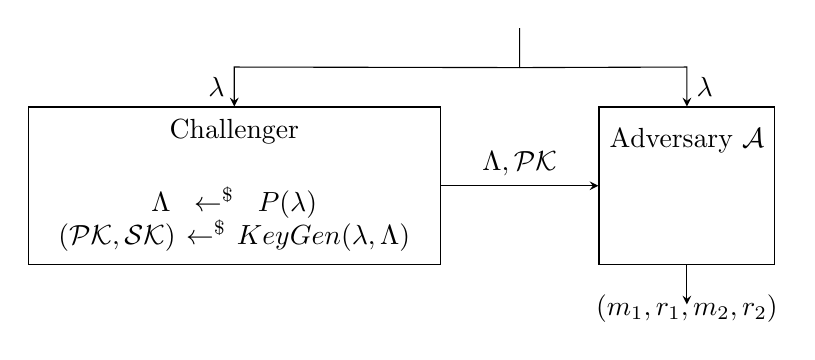
\begin{tikzpicture}[>=stealth]
  %coordinates
  \coordinate (orig) at (0,0);
  % Nodes
  \node[draw, minimum width=5cm, minimum height=2cm, anchor=east, text width=5cm, align=center](C) at (0,0) {Challenger\vskip5mm$\Lambda\leftarrow^{\$}P(\lambda)$\\$(\mathcal{PK}, \mathcal{SK}) \leftarrow^{\$}KeyGen(\lambda, \Lambda)$};
  \node[draw, anchor=west, minimum height=2cm,text width=2cm, align=center](A) at (2,0){Adversary $\mathcal{A}$\vskip8mm\ };
  % Edges
  \path[draw,->] (1,2) -- (1,3/2) -- ($(C.90) + (0,1/2)$) -- node[left]{$\lambda$} (C.90);
  \path[draw,->](1,3/2) -- ($(A.90) + (0, 1/2)$) -- node[right]{$\lambda$} (A.90);
  \draw[->](C.0)--node[above]{$\Lambda, \mathcal{PK}$}(A.180);
  \draw[->](A.270)--node[below]{$(m_1, r_1, m_2, r_2)$} ($(A.270) - (0, 1/2)$);
  \end{tikzpicture} 
 \caption{Attack Game 1: Collision Resistance. Adversary $\mathcal{A}$ wins if $(m_1, r_1)\neq(m_2, r_2)$ and $Hash(m_1, r_1)=Hash(m_2, r_2)$.}
 \end{figure}
 \end{game}
 
 \begin{definicao}
 We call a chameleon hash scheme \textbf{collision resistent} if for
 all efficient adversaries $\mathcal{A}$,
 $Adv_{ColRes}[\mathcal{A},CH](\lambda)$ is a negligible
 function.
 \end{definicao}
 
 We notice that a chameleon hash scheme can't be collision resistant if
 $|C_{\lambda,\Lambda}|$ isn't superpolynomial with respect to
 $\lambda$, as
 a naive attacker whitch chooses random values of $(m_1, r_1, m_2,
 r_2)$ succeds with probability $1/|C_{\lambda,\Lambda}|$.
 
 \begin{game}
 \textbf{Preimage Resistance: }For a given chameleon hash scheme $CH$
 defined over $(M, R, C)$, and an adversary $\mathcal{A}$,
 a challenger sends to the adversary $\lambda$, $\Lambda$,
 $\mathcal{PK}$ and $c \in C_{\lambda,\Lambda}$ and the adversary
 outputs $m' \in M_{\lambda,\Lambda}$ and $r' \in R_{\lambda,\Lambda}$.
 
 We say that the adversary $\mathcal{A}$ wins the game if
 $Hash(\lambda, \Lambda, \mathcal{PK}, m', r') = c$
 
 We define $\mathcal{A}$'s advantage with respect to $CH$ as the
 function whitch outputs the probability that $\mathcal{A}$ wins 
 game given $\lambda$. We denote this advantage as
 $Adv_{PreImg}[\mathcal{A},CH](\lambda)$.
 
 \begin{figure}
 \centering
   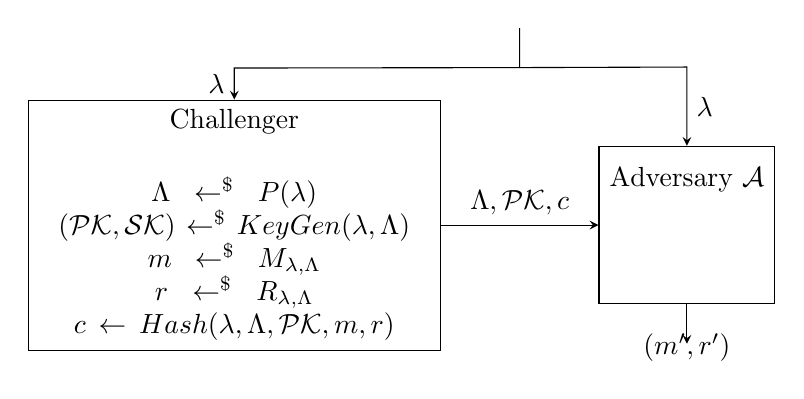
\begin{tikzpicture}[>=stealth]
  % Nodes
  \node[draw, minimum width=5cm, minimum height=2cm, anchor=east, text width=5cm, align=center](C) at (0,0) {Challenger\vskip5mm$\Lambda\leftarrow^{\$}P(\lambda)$\\$(\mathcal{PK}, \mathcal{SK}) \leftarrow^{\$}KeyGen(\lambda, \Lambda)$\\$m\leftarrow^{\$}M_{\lambda,\Lambda}$\\$r\leftarrow^{\$}R_{\lambda,\Lambda}$\\$c\leftarrow Hash(\lambda,\Lambda,\mathcal{PK},m, r)$};
  \node[draw, anchor=west, minimum height=2cm,text width=2cm, align=center](A) at (2,0){Adversary $\mathcal{A}$\vskip8mm\ };
  % Edges
  \path[draw,->] (1,5/2) -- (1,2) -- ($(C.90) + (0,0.4)$) -- node[left]{$\lambda$} (C.90);
  \path[draw,->](1,2) -- ($(A.90) + (0, 1)$) -- node[right]{$\lambda$} (A.90);
  \draw[->](C.0)--node[above]{$\Lambda, \mathcal{PK}, c$}(A.180);
  \draw[->](A.270)--node[below]{$(m', r')$} ($(A.270) - (0, 1/2)$);
  \end{tikzpicture} 
 \caption{Attack Game 2: Preimage Resistance. Adversary $\mathcal{A}$ wins if $Hash(m', r')=c$.}
 \end{figure}
 \end{game}
 
 \begin{definicao}
 We call a chameleon hash scheme \textbf{preimage resistent} 
 or an \textbf{one-way function} if for all efficient adversaries
 $\mathcal{A}$, $Adv_{PreImg}[\mathcal{A},CH](\lambda)$ is a negligible
 function.
 \end{definicao}
 
 We can define a related property of \textbf{second-preimage
 resistance} with the following attack game:
 
 \begin{game}
 \textbf{Second-Preimage Resistance: }For a given chameleon hash scheme
 $CH$ defined over $(M, R, C)$, and an adversary $\mathcal{A}$,
 a challenger sends to the adversary $\lambda$, $\Lambda$,
 $\mathcal{PK}$, $m \in M_{\lambda,\Lambda}$ and 
 $r \in R_{\lambda,\Lambda}$ and the adversary
 outputs $m' \in M_{\lambda,\Lambda}$ and $r' \in R_{\lambda,\Lambda}$.
 
 We say that the adversary $\mathcal{A}$ wins the game if
 $Hash(\lambda, \Lambda, \mathcal{PK}, m', r') = 
 Hash(\lambda, \Lambda, \mathcal{PK}, m, r)$ and $(m, r) \neq (m', r')$.
 
 We define $\mathcal{A}$'s advantage with respect to $CH$ as the
 function whitch outputs the probability that $\mathcal{A}$ wins 
 game given $\lambda$. We denote this advantage as
 $Adv_{2PreImg}[\mathcal{A},CH](\lambda)$.
 
 \begin{figure}
 \centering
    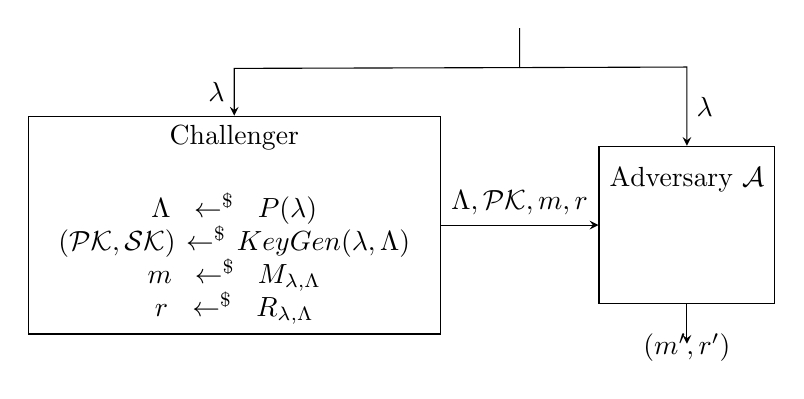
\begin{tikzpicture}[>=stealth]
  % Nodes
  \node[draw, minimum width=5cm, minimum height=2cm, anchor=east, text width=5cm, align=center](C) at (0,0) {Challenger\vskip5mm$\Lambda\leftarrow^{\$}P(\lambda)$\\$(\mathcal{PK}, \mathcal{SK}) \leftarrow^{\$}KeyGen(\lambda, \Lambda)$\\$m\leftarrow^{\$}M_{\lambda,\Lambda}$\\$r\leftarrow^{\$}R_{\lambda,\Lambda}$};
  \node[draw, anchor=west, minimum height=2cm,text width=2cm, align=center](A) at (2,0){Adversary $\mathcal{A}$\vskip8mm\ };
  % Edges
  \path[draw,->] (1,5/2) -- (1,2) -- ($(C.90) + (0,0.6)$) -- node[left]{$\lambda$} (C.90);
  \path[draw,->](1,2) -- ($(A.90) + (0, 1)$) -- node[right]{$\lambda$} (A.90);
  \draw[->](C.0)--node[above]{$\Lambda, \mathcal{PK}, m, r$}(A.180);
  \draw[->](A.270)--node[below]{$(m', r')$} ($(A.270) - (0, 1/2)$);
  \end{tikzpicture} 
 \caption{Attack Game 3: Second-Preimage Resistance. Adversary $\mathcal{A}$ wins if $(m, r)\neq(m', r')$ and $Hash(m, r)=Hash(m', r')$.}
 \end{figure}
 \end{game}
 
 \begin{definicao}
 We call a chameleon hash scheme \textbf{second-preimage resistent} 
 if for all efficient adversaries $\mathcal{A}$,
 $Adv_{2PreImg}[\mathcal{A},CH](\lambda)$ is a negligible
 function.
 \end{definicao}
 
 Unlike in usual hash functions, in chameleon hashes, all pairs
 of possible input $(m, r)$ have a second-preimage. The existance 
 of functions $Collision$ and $PreImage$ guarantees this. From 
 $Collision$ and $PreImage$ function definitions,
 given any pair $(m, r)$, we can find at least $|M_{\lambda,\Lambda}|-1$
 second-preimages.
 
 This shows that the number of different input for our $Hash$ function
 is at least the number of possible digests multiplied by the number
 of possible messages: $|M_{\lambda,\Lambda}|.|R_{\lambda,\Lambda}|
 \geq |M_{\lambda,\Lambda}|.|C_{\lambda,\Lambda}|$. So the number
 of different random parameters must always be at least the same as the
 number of different digests.
 
 \begin{theorem}
 If a chameleon hash scheme is collision resistant, then it's also
 second-preimage resistant.
 \end{theorem}
 
 \textbf{Proof:} We will prove that if the chameleon hash is not
 second-preimage resistant, then it's also not collision resistant.
 
 If exists some efficient adversary $\mathcal{A}$ which can win the
 attack game 3 with non-negligible probability, then we can build an
 efficient adversary $\mathcal{B}$ which can win the Attack Game 1 with
 non-negligible probability.
 
 The adversary $\mathcal{B}$ gets $\lambda$, $\Lambda$ and 
 $\mathcal{PK}$ as input. It can then generate 
 $m \leftarrow^{\$}M_{\lambda, \Lambda}$ and 
 $r \leftarrow^{\$}R_{\lambda,\Lambda}$
 and pass all these values as input to $\mathcal{A}$. I gets $(m', r')$
 from $\mathcal{A}$'s output and returns $(m, r, m', r')$.
 
 We have:
 
 $$
 Adv_{ColRes}[B, CH](\lambda) = Adv_{2PreImg}[A, CH](\lambda)
 $$
 
 So exists such efficient $\mathcal{B}$ given that $\mathcal{A}$ exists.
 \qed
 
 \begin{theorem}
 If for a chameleon hash scheme is second-preimage resistant, then 
 it's also preimage resistant.
 \end{theorem}
 
 \textbf{Proof:} We will show that if we find an adversary $\mathcal{A}$
 which could win the Attack Game 2 with non-negligible probability,
 we could build an adversary $\mathcal{B}$ which uses $\mathcal{A}$
 to win the attack game for second-preimage resistance.
 
 Our adversary $\mathcal{B}$ just get $\lambda$ and 
 $(\Lambda,\mathcal{PK}, m, r)$ as input and then computes
 $c=Hash(\lambda, \Lambda, \mathcal{PK}, m, r)$. It then passes
 $\lambda$ and $(\Lambda, \mathcal{PK}, c)$ to adversary $\mathcal{A}$.
 Then it collects and return as output $\mathcal{A}$'s output.
 
 As all the pairs $(m, r)$ always have at least $|M_{\lambda,\Lambda}|$
 preimages, if $\mathcal{A}$ returns a correct output, the only
 case when $\mathcal{B}$ wouldn't win the game would be if
 $(m, r) = (m', r')$. This happens with probability
 $1/|M_{\lambda,\Lambda}|$ in the worst case.
 So:
 
 $$
 \left(1-\frac{1}{|M_{\lambda,\Lambda}|}\right)
 Adv_{PreImg}[\mathcal{A},CH](\lambda) \leq Adv_{2PreImg}[\mathcal{B},CH](\lambda)
 $$
 
 So we conclude that if $\mathcal{A}$ wins with non-negligible probability, then $\mathcal{B}$
 would also win with non-negligible probability. \qed
 
 The previous theorem isn't necessarily true for traditional
 cryptographic hash functions, mainly because for them we can't
 guarantee that all possible inputs have a second-preimage.
 
 We also need the property that a digest doesn't reveal any information
 about the message. We define this with the semantic security property.
 
 \begin{game}
 \textbf{Semantic Security: }For a given chameleon hash scheme $CH$
 defined over $(M, R, C)$, and for a given adversary $\mathcal{A}$,
 we define two experiments: Experiment 0 and Experiment 1. For $b=0,1$,
 in Experiment $b$ the adversary computes 
 $m_0, m_1 \in M_{\lambda,\Lambda}$ and sends them to the challenger.
 The challenger chooses uniformly a $r \in R_{\lambda,\Lambda}$
 and sends $Hash(m_b, r)$ to the adversary. The adversary outputs a
 bit $\hat b\in \{0,1\}$.
 
 For $b=0,1$, let $W_b$ be the event that the adversary outputs
 1 in experiment $b$. We define $\mathcal{A}$'s semantic security
 advantage with respect to $CH$ as:
 
 $$
 Adv_{SS}[\mathcal{A}, CH](\lambda) = |Pr[W_0]-Pr[W_1]|
 $$
 
 \begin{figure}
 \centering
    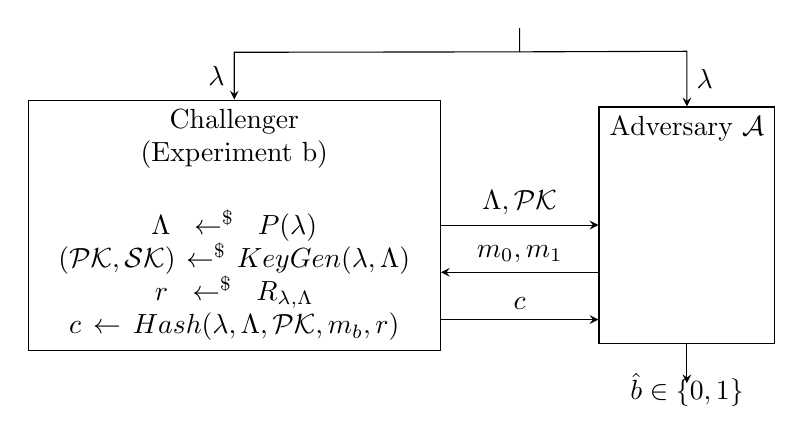
\begin{tikzpicture}[>=stealth]
  % Nodes
  \node[draw, minimum width=5cm, minimum height=3cm, anchor=east, text width=5cm, align=center](C) at (0,0) {Challenger\\(Experiment b)\vskip5mm$\Lambda\leftarrow^{\$}P(\lambda)$\\$(\mathcal{PK}, \mathcal{SK}) \leftarrow^{\$}KeyGen(\lambda, \Lambda)$\\$r\leftarrow^{\$}R_{\lambda,\Lambda}$\\$c\leftarrow Hash(\lambda, \Lambda, \mathcal{PK}, m_b, r)$};
  \node[draw, anchor=west, minimum height=3cm,text width=2cm, align=center](A) at (2,0){Adversary $\mathcal{A}$\vskip2.1cm\ };
  % Edges
  \path[draw,->] (1,5/2) -- (1,2.2) -- ($(C.90) + (0,0.6)$) -- node[left]{$\lambda$} (C.90);
  \path[draw,->](1,2.2) -- ($(A.90) + (0, 0.7)$) -- node[right]{$\lambda$} (A.90);
  \draw[->](C.0)--node[above]{$\Lambda, \mathcal{PK}$}(A.180);
  \draw[->]($(A.180) - (0, 0.6)$)--node[above]{$m_0, m_1$}($(C.0) - (0,0.6)$);
  \draw[->]($(C.0) - (0, 1.2)$)--node[above]{$c$}($(A.180) - (0,1.2)$);
  \draw[->](A.270)--node[below]{$\hat{b}\in\{0,1\}$} ($(A.270) - (0, 1/2)$);
  \end{tikzpicture} 
  %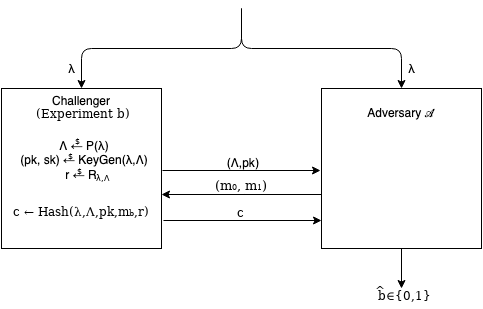
\includegraphics[width=0.9\textwidth]{imagens/semantic.png}
 \caption{Attack Game 4: Semantic Security. The adversary $\mathcal{A}$ wins if it outputs different values in Experiment 0 ($b=0$) and Experiment 1 ($b=1$).}
 \end{figure}
 \end{game}
 
 \begin{definicao}
 We call a chameleon hash scheme \textbf{semantically secure} 
 if for all efficient adversaries $\mathcal{A}$,
 $Adv_{SS}[\mathcal{A},CH](\lambda)$ is a negligible function.
 \end{definicao}
 
 For chameleon hashes, any possible message can produce any possible
 digest, given the correct random parameter. But the semantic security
 ensures that some digests aren't more probable for some messages than
 for others. Otherwise an adversary could identify if a random 
 parameter was chosen randomly or was produced with a $Collision$ or
 $PreImage$ function. We could assume that an improbable digest for a
 given message was created with a parameter returned by $Collision$
 or $PreImage$, not chosen randomly.
 
 The previous security definitions are necessary, but still 
 insufficient to model realistic scenarios of chameleon hash usage. 
 Unlike regular hash functions, here we have the algorithms
 $Collision$ and $PreImage$ which could be used to create
 publicly known examples of collisions. An attacker could also
 induce the owner of a private key to create a desired
 collision. To represent these requirements, the security definitions
 must be strengthened allowing an adversary to query for examples
 of collisions or preimages.
 
 All the previous definitions can be defined under this stronger attack model. This is analogous as how encription can be defined under the chosen plaintext model, where an attacker can query the challenger for examples of encription. But here, as we are dealing with collisions of hash messages, we will call this attack model the \textbf{chosen collision attack}.
 
 \begin{definicao}
 A security property defined for a chameleon hash $CH$ as the advantage of adversaries under an attack game is said under \textbf{chosen collision attack} if in its attack game, before returning the final output, the adversary can make $Q$ queries in the following formats:
 \begin{itemize}
     \item For query $i$, the Adversary sends $(m_i, r_i, m'_i)$ with $m_i, m'i \in M_{\lambda,\Lambda}$ and $r_i\in R_{\lambda,\Lambda}$. The Challenger reply with $r'_i$ such as $r_i = Collision(\lambda, \Lambda, \mathcal{SK}, m_i, r_i, m'_i)$.
     \item For query $i$, the Adversary sends $(m_i, c_i)$ and the Challenger reply with $r_i = PreImage(\lambda, \Lambda, \mathcal{SK}, m_i, c_i)$ if $CH$ is a Preimage Chameleon Hash, or reply with ``\texttt{unknown}'' otherwise.
     \item If the property already required the adversary to query values (like in the Semantic Security Attack Game, when the adversary sends $m_1, m_2$), now the adversary can also repeat this query with other values (in Semantic Security under Chosen Collision the adversary can send queries $(m_{0i}, m_{1i})$ and get as answer $c_i$ such as $c_i=Hash(m_{bi}, r)$).
     \end{itemize}
     
     Such queries are adaptative, the Adversary can choose each one after analyzing the previous queries result.
     
     After the queries, if the adversary outputs any pair $(m, r)$, for $m\in M_{\lambda,\Lambda}$ or $R_{\lambda, \Lambda}$, at least one of these pairs $(m, r)$ must have the property that $(m, r)\neq (m_i, r_i)$ and $(m, r)\neq(m'_i, r'_i)$ for all $i \in \{1, \ldots, Q\}$.

     If an adversary $\mathcal{A}$ have some advantage $P_{ADV}[\mathcal{A}, CH]$ in a weaker attack model, we say that it has the advantage $P_{ADV}^{CC}[\mathcal{A}, CH]$ under the chosen collision attack.
          
     As an example, Figure \ref{fig:chosencol} shows the Attack Game of Collision Resistance under Chosen Collision Attack.
     
     \begin{figure}
     \label{fig:chosencol}
 \centering
  %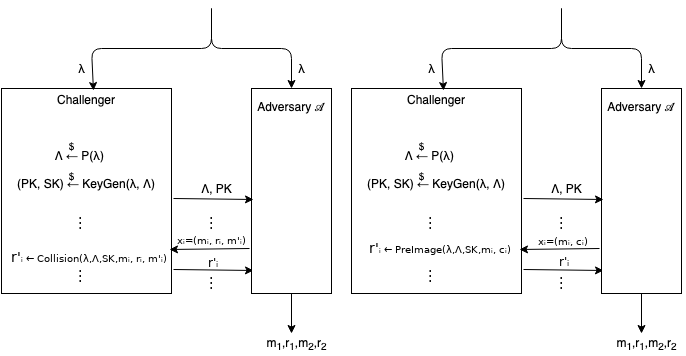
\includegraphics[width=0.95\textwidth]{imagens/col_res_cc.png}
  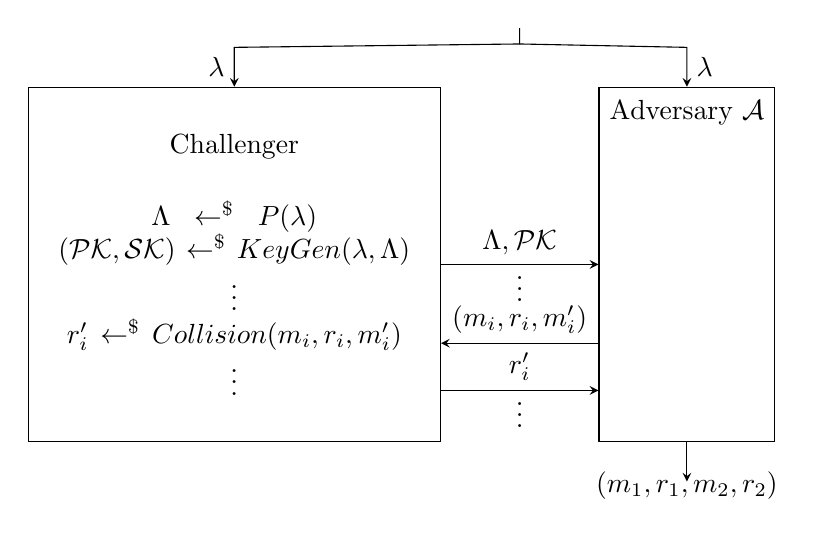
\begin{tikzpicture}[>=stealth]
  %coordinates
  \node[draw, minimum width=5cm, minimum height=4.5cm, anchor=east, text width=5cm, align=center](C) at (0,0) {Challenger\vskip5mm$\Lambda\leftarrow^{\$}P(\lambda)$\\$(\mathcal{PK}, \mathcal{SK}) \leftarrow^{\$}KeyGen(\lambda, \Lambda)$\\$\vdots$\\$r'_i\leftarrow^{\$} Collision(m_i, r_i, m'_i)$\\$\vdots$};
  \node[draw, anchor=west, minimum height=2cm, minimum height=4.5cm, text width=2cm, align=center](A) at (2,0){Adversary $\mathcal{A}$\vskip3.5cm\ };
  % Edges
  \path[draw,->] (1,3) -- (1,2.8) -- ($(C.90) + (0,1/2)$) -- node[left]{$\lambda$} (C.90);
  \path[draw,->](1,2.8) -- ($(A.90) + (0, 0.5)$) -- node[right]{$\lambda$} (A.90);
  \draw[->](C.0)--node[above]{$\Lambda, \mathcal{PK}$}(A.180);
  \path($(C.0)-(0,0.6)$)--node[above]{$\vdots$}($(A.180)-(0,0.6)$);
\draw[->]($(A.180)-(0,1)$)--node[above]{$(m_i, r_i, m'_i)$}($(C.0)-(0,1)$);
\draw[->]($(C.0)-(0,1.6)$)--node[above]{$r'_i$}($(A.180)-(0,1.6)$);
\path($(C.0)-(0,2.2)$)--node[above]{$\vdots$}($(A.180)-(0,2.2)$);
  \draw[->](A.270)--node[below]{$(m_1, r_1, m_2, r_2)$} ($(A.270) - (0, 1/2)$);
  \end{tikzpicture} 
 \caption{Example of Attack Game under Chosen Collision Attack: Collision Resistance under Chosen Collision Attack. The adversary $\mathcal{A}$ wins if after making $Q$ queries $(m_i, r_i, m'_i)$ with $i \in \{1, \ldots, Q\}$, it outputs $(m_1, r_1, m_2, r_2)$ such as $(m_1, r_1)\neq(m_2, r_2)$, $(m_2, r_2)\neq(m_i, r_i)$ and $(m_2, r_2)\neq(m'_i, r'_i)$ for all $i \in \{1, \ldots, Q\}$.}
 \end{figure}
 \end{definicao}
 
 This is our strongest attack model. It's easy to see that any chameleon hash collision resistant under chosen collision attack is also collision resistant under the weaker attack model. The converse isn't true. If you reveal for an adversary that $r'=Collision(m, r, m')$, this leaks information. In the worst case, the adversary can use this to extract the challenger's private key. If this happens, the chameleon hash isn't collision resistant nor second-preimage resistant under chosen collision attack, even if it has these properties in the weaker model.
 
 Not always this strong attack model is ideal. In some chameleon hash applications, it's desired to be able to compute collisions even without the private key if we have previous examples of collisions which result in the same digest. This happens in Chameleon Signatures Schemes. Some important chameleon hash constructions can also be insecure under chosen collision attack, but secure under new and intermediate attack models. If necessary, we define other attack models when presenting these applications and constructions.
 
 \begin{theorem}
 If for a chameleon hash scheme $CH$, if $|R_{\lambda, \Lambda}|$ is superpolynomial and for all tuples $(c, m_1, m_2)$ with $c \in C_{\lambda, \Lambda}$ and $m_1, m_2 \in M_{\lambda, \Lambda}$, the number of random parameters $r_1\in R_1$ such as $Hash(m_1, r_1)=c$ and $r_2\in R_2$ such as $Hash(m_2, r_2)=c$, if $|R_1| \approx |R_2|$, then $CH$ is semantically secure and is also semantically secureunder chosen collision attack. 
 \end{theorem}
 
 \textbf{Proof:} TODO. \qed
 
\section{Construção Baseada em Permutações de Resíduos Qua\-drá\-ti\-cos (Krawczyk) (2000) \cite{krawczyk}}

 \subsection{Funções}
 
 \textbf{KeyGen: }Como chave pública, gere duas funções de permutação
 que atuam sobre um mesmo Domínio. Chamaremos elas de $f_0$ e
 $f_1$. Como chave privada, armazene o inverso destas funções:
 $f_0^{-1}$ e $f_1^{-1}$.
 
 A construção de Krawczyk usa como funções: $f_0(x) = x^2 \mod n$ e
 $f_1(x) = 4x^2 \mod n$ para $n$ sendo um múltiplo de dois primos
 grandes $p$ e $q$, tal que $p \equiv 3 \mod 8$ e $q \equiv 7 \mod
 8$. E sendo a função definida apenas para resíduos quadráticos módulo
 $n$ que também são primos em relação à $n$. A chave pública precisa
 então apenas armazenar $n$ e a chave privada armazena $p$ e $q$. As
 funções inversas envolvem raíz quadrada modular, as quais só sabemos
 como resolver eficientemente módulo $n$ quando conhecemos os fatores
 de $n$.
 
 \textbf{Hash:} A função aceita como parâmetro aleatório somente
 valores de $r$ que são resíduos quadráticos módulo $n$. Em seguida,
 usando a representação binária da mensagem $m$, percorremos em ordem
 cada um dos bits em uma iteração. Inicialmente o valor do hash é
 considerado como igual a $r$. Em cada bit da iteração atualizamos como
 novo valor da hash o valor anterior passado para $f_0$ se o bit for 0
 ou o valor anterior passado para $f_1$ se o bit for 1.
 
 \textbf{PreImage:} Para obter um valor válido de $r$ para que a
 mensagem $m$ tenha o hash $C$, comece com o valor inicial de $C$ e
 percorra a representação binária de $m$ de trás pra frente. Toda vez
 que encontrar um 0, aplique sobre o valor atual de $r$ a função
 $f_0^{-1}$. Sempre que encontrar um 1, aplique $f_1^{-1}$. O valor
 final é o $r$ desejado.
 
 \textbf{Collision:} Basta escolher uma mensagem $m'$ qualquer que seja
 diferente de $m$ e calcular usando a equação:
 
 $Collision(\mathcal{SK}, m, r) = (m', PreImage(\mathcal{SK}, m',
 Hash(\mathcal{PK}, m, r)))$
 
 Isso funciona pelo fato de que toda mensagem neste esquema é capaz de
 produzir qualquer $c \in C$, bastando que se mude o valor de $r$
 utilizado no hash.
 
 \subsection{A Exposição de Chave}
 
 Se encontramos uma colisão nesta hash camaleão, temos duas mensagens
 que à partir de algum momento em que iteramos sobre seus bits, obtemos
 valores distintos $x$ e $y$ tais que:
 
 $$
 x^2 \equiv 4y^2 \pmod n
 $$
 
 O que nos leva a:
 
 $$
 x^2 - 4y^2 \equiv 0 \pmod n
 $$
 
 $$
 (x+2y)(x-2y) \equiv 0 \pmod n
 $$
 
 Desta forma, conseguimos fatorar $n$ e ter acesso à chave privada
 $\mathcal{SK}$.
 
 O mesmo raciocínio também nos mostra que encontrar uma colisão sem
 acesso à $\mathcal{SK}$ é tão difícil quanto fatorar números.
 
 %\subsection{Propriedades}
 
 %As seguintes propriedades são específicas da construção de Krawczyk. O
 %uso de diferentes permutações pode mudar as propriedades.
 
 %\textbf{Resistência a Colisão: }Sim se assumirmos que é difícil
 %fatorar números.
 
 %\textbf{Ocultação de Mensagem: }Sim, usando a função \textbf{IForge}
 %definida acima.
 
 %\textbf{Livre de Exposição de Chave: } Não.
 
 %\textbf{Cálculo de Primeira Pré-Imagem: }Sim.
 
 \subsection{Exemplo Didático}
 
 Começamos escolhendo os valores $p=3$ e $q=7$, que tem a propriedade
 desejada de serem respectivamente côngruos a 3 e 7 módulo
 8. Multiplicamos estes números para obtermos $n = 21 = pq$. No módulo
 21 obtemos 3 números que são resíduos quadráticos: 1, 4 e 16.
 
 Com estes três valores diferentes, definimos a função $f_0(x)=x^2\mod
 21$ e $f_1=4x^2\mod 21$:
 
 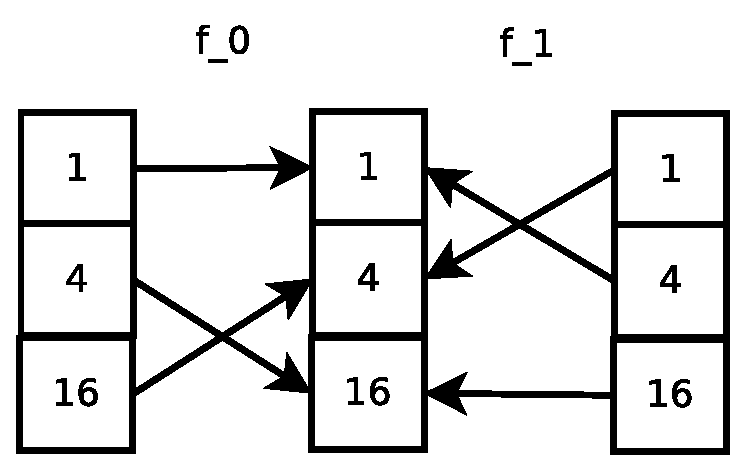
\includegraphics[width=5cm]{imagens/toy1.eps}
 
 Para gerarmos o hash da mensagem com bits $01101$, geramos um $r$
 aleatório que pode ser 1, 4 ou 16. No caso, escolhemos 4. Calculamos
 então:
 
 $$
 f_1(f_0(f_1(f_1(f_0(4))))) = f_1(f_0(f_1(f_1(16)))) = f_1(f_0(f_1(16))) =
 f_1(f_0(16)) = f_1(4) = 1
 $$
 
 Queremos que a mensagem com bits $00101$ tenha exatamente o mesmo hash
 que a mensagem acima (no caso, 1). Para descobrirmos o valor de $r'$
 que devemos associar à ela para este fim, calculamos:
 
 $$
 f_0^{-1}(f_0^{-1}(f_1^{-1}(f_0^{-1}(f_1^{-1}(1))))) =
 f_0^{-1}(f_0^{-1}(f_1^{-1}(f_0^{-1}(4)))) =
 f_0^{-1}(f_0^{-1}(f_1^{-1}(16))) =
 $$
 $$
 =f_0^{-1}(f_0^{-1}(16)) = f_0^{-1}(4) = 16
 $$
 
 O que significa que podemos calcular o hash dessa mensagem e obteremos
 $Hash(00101, 16)=1$. O que podemos conferir calculando abaixo:
 
 $$
 f_1(f_0(f_1(f_0(f_0(16))))) = f_1(f_0(f_1(f_0(4)))) = f_1(f_0(f_1(16))) =
 f_1(f_0(16)) = f_1(4) = 1
 $$
 
 Exatamente o valor que era esperado.
 
 \subsection{Medida de Desempenho}
 
 Usando uma implementação em C baseada na biblioteca GNU MP com chaves
 de 2048 bits e mensagens de 54 bytes, rodando em um computador Intel
 i7, foi obtido os seguintes tempos de execução:
 
 \begin{center}
 \begin{tabular}{|c|c|c|c|c|c|}
 \hline
 KeyGen & 0,43400s & Hash & 0,00104s & Collision & 1,79000s\\
 \hline
 \end{tabular}
 \end{center}
 
 
 \section{Construção Baseada em Logaritmo Discreto (Krawczyk) (2000)
 \cite{krawczyk}}
 
 \subsection{Funções}
 
 \textbf{KeyGen: }Primeiro encontre primos grandes $p$ e $q$ tais que
 $p = kq+1$ e um grupo multiplicativo modular $\mathbb{Z}^{*}_p$ com um
 gerador $g$.
 
 A chave privada é um valor aleatório $x \in \mathbb{Z}^{*}_q$.
 
 A chave pública é um valor $y = g^x \mod p$.
 
 \textbf{Hash:}Dada uma mensagem $m \in \mathbb{Z}^{*}_q$ e um
 parâmetro $r\in \mathbb{Z}^{*}_q$, a hash camaleão é obtida por meio
 da definição:
 
 $$
 Hash(\mathcal{PK}=y, m, r) = g^my^r \mod p
 $$
 
 \textbf{PreImage:} Não. Seria necessário resolver o problema do
 logaritmo discreto para implementar esta função.
 
 \textbf{Collision:} A chave privada é o logaritmo discreto de $y$. Se
 temos um $m$ e um $r$ que possui um hash conhecido e queremos que um
 $m'$ qualquer gere o mesmo valor hash, o valor $r'$ necessário é
 retornado por:
 
 $$
 Collision(\mathcal{SK}=x, m, r, m') = (m+xr-m')(x)^{-1}
 $$
 
 Este esquema não é livre de exposição de chaves. A chave secreta $x$
 pode ser obtida por qualquer um que tenha acesso à uma colisão $(m,
 r)$ e $(m', r')$ por meio da fórmula $m+xr = m'+xr'$.
 
 %\subsection{Propriedades}
 
 %\textbf{Resistência a Colisão: }Sim se assumirmos que é difícil
 %calcular o logaritmo discreto no grupo escolhido.
 
 %\textbf{Ocultação de Mensagem: }Sim, usando a função \textbf{IForge}.
 
 %\textbf{Livre de Exposição de Chave: } Não.
 
 %\textbf{Cálculo de Primeira Pré-Imagem: }Não.
 
 \subsection{Exemplo Didático}
 
 Vamos escolher um $p=11=(5)(2)+1$ com um $q=5$. Para o nosso valor de
 $p$ temos então o seguinte grupo multiplicativo:
 
 \begin{tabular}{|c||c|c|c|c|c|c|c|c|c|c|}
 \hline
 $\times$&1&2&3&4&5&6&7&8&9&10\\
 \hline
 \hline
 1&1&2&3&4&5&6&7&8&9&10\\
 \hline
 2&2&4&6&8&10&1&3&5&7&9\\
 \hline
 3&3&6&9&1&4&7&10&2&5&8\\
 \hline
 4&4&8&1&5&9&2&6&10&3&7\\
 \hline
 5&5&10&4&9&3&8&2&7&1&6\\
 \hline
 6&6&1&7&2&8&3&9&4&10&5\\
 \hline
 7&7&3&10&6&2&9&5&1&8&4\\
 \hline
 8&8&5&2&10&7&4&1&9&6&3\\
 \hline
 9&9&7&5&3&1&10&8&6&4&2\\
 \hline
 10&10&9&8&7&6&5&4&3&2&1\\
 \hline
 \end{tabular}
 
 Com relação à exponenciação, se fizermos o valor de cada linha abaixo
 elevado ao valor da coluna obtemos a tabela:
 
 \begin{tabular}{|c||c|c|c|c|c|c|c|c|c|c|}
 \hline
 $a^b$&1&2&3&4&5&6&7&8&9&10\\
 \hline
 \hline
 1&1&1&1&1&1&1&1&1&1&1\\
 \hline
 2&2&4&8&5&10&9&7&3&6&1\\
 \hline
 3&3&9&5&4&1&3&9&5&4&1\\
 \hline
 4&4&5&9&3&1&4&5&9&3&1\\
 \hline
 5&5&3&4&9&1&5&3&4&9&1\\
 \hline
 6&6&3&7&9&10&5&8&4&2&1\\
 \hline
 7&7&5&2&3&10&4&6&9&8&1\\
 \hline
 8&8&9&6&4&10&3&2&5&7&1\\
 \hline
 9&9&4&3&5&1&9&4&3&5&1\\
 \hline
 10&10&1&10&1&10&1&10&1&10&1\\
 \hline
 \end{tabular}
 
 Podemos escolher qualquer elemento cuja ordem é $q=5$ como
 gerador. Pode ser o 3, 4, 5 ou 9. Escolheremos então $g=5$. Podemos
 escolher como chave privada os valores 1, 2, 3 ou 4, pois eles tem
 ordem $q=5$. Façamos então $\mathcal{SK}=3$. O que faz com que nossa
 chave pública seja $\mathcal{PK}=5^3\mod 11 = 4$.
 
 Vamos calcular um hash para a mensagem representada pelo número
 $m=8$. O nosso parâmetro aleatório $r$ pode ser 1, 2, 3 ou 4. Façamos
 então $r=2$. A hash é calculada então por:
 
 $$
 Hash(\mathcal{PK}=4, m=8, r=2) = g^my^r = 5^84^2 \mod 11 = 9
 $$
 
 Agora supondo que tenhamos a chave privada, queremos fazer com que a
 mensagem $m'=7$ tenha exatamente o mesmo valor de hash. Para isso
 fazemos:
 
 \begin{equation}
 \begin{split}
 UForge(\mathcal{SK}=3, m=8, r=2, m'=7) &= \frac{m+xr-m'}{x} \mod 5\\
 &= 2(3)^{-1} \mod 5 = (2)(2) \mod 5 = 4
 \end{split}
 \end{equation}
 
 Para checar que isso é correto, vamos calcular:
 
 $$ Hash(\mathcal{PK}=4, m'=7, r'=4) = g^{m'}y^{r'} = 5^74^4 \mod 11 =
 (3)(3)= 9
 $$
 
 Exatamente o resultado esperado.
 
 \subsection{Medida de Desempenho}
 
 \begin{center}
 \begin{tabular}{|c|c|c|c|c|c|}
 \hline
 KeyGen & 0,005490s & Hash & 0,009530s & Collision & 0,000032s\\
 \hline
 \end{tabular}
 \end{center}
 
 \section{Construção Baseada em Assinaturas Nyberg-Rueppel
 (Ateniese e Medeiros) (2005)\cite{ateniese2004key}}
 
 Esta construção se baseia na existência do esquema de assinaturas
 Nyberg-Rueppel, um dos esquemas baseados no ElGamal. Nele, começamos
 gerando dois números primos $p$ e $q$ tais que $p=2q+1$. Escolhemos
 também um gerador $g$ do subgrupo de resíduos quadráticos de
 $\mathbb{Z}_p$ de ordem $q$. Escolhemos como chave privada um número
 $x$ módulo $q$ e escolhemos como chave pública um valor $y=g^x \mod
 p$.
 
 Em uma das variações dessa assinatura, assinar uma mensagem $m$ é
 feito por meio da equação:
 
 $$
 Sign(m) = (r, s) = ((g^k \mod p) \mod q, k-rmx \mod q)
 $$
 
 E uma assinatura $(r, s)$ é válida para uma mensagem $m$ se:
 
 $$
 r = (g^sy^{rm} \mod p) \mod q
 $$
 
 O valor $k$ acima deve ser sempre escolhido aleatoriamente e não pode
 ser revelado, ou a chave privada poderia ser facilmente extraída.
 
 A ideia será gerar um esquema de hash camaleão no qual a equação de
 verificação acima será usada para o nosso hash e a equação de
 assinatura será usada para obter uma pré-imagem após fazermos algumas
 modificações. A única mudança que precisará ser feita será a
 substituição do produto $mr$ pelo resultado do hash convencional
 $\mathcal{H}(m||r)$ em todas as equações acima. Desta forma, ficaremos
 com as equações abaixo que servirão de base para nosso hash camaleão.
 
 Equações de verificação:
 
 $$
 r = (g^k \mod p) \mod q
 $$
 
 $$
 s = k-\mathcal{H}(m||r)x \mod q
 $$
 
 Equação de assinatura:
 
 $$
 r = (g^sy^{\mathcal{H}(m||r)} \mod p) \mod q
 $$
 
 \textbf{A Compreender: }Por que foi necessário fazer a substituição de
 $mr$ por $\mathcal{H}(m||r)$? A rigor, o esquema continuaria
 funcionando se essa substituição não tivesse sido feita.
 
 \subsection{Funções}
 
 \textbf{KeyGen: }A geração de chaves é idêntica à do esquema de
 assinatura. Começamos gerando dois números primos $p$ e $q$ tais que
 $p=2q+1$. Escolhemos também um gerador $g$ do subgrupo de resíduos
 quadráticos de $\mathbb{Z}_p$ de ordem $q$. Escolhemos como chave
 privada um número $x$ módulo $q$ e escolhemos como chave pública um
 valor $y=g^x \mod p$.
 
 \textbf{Hash: } Geraremos uma função de hash que será baseada na
 verificação para saber se uma assinatura Nyberg-Rueppel é válida para
 uma mensagem $m$. Nosso hash será definido como:
 
 $$
 Hash(m, (r, s)) = r - (g^sy^{\mathcal{H}(m, r)} \mod p) \mod q
 $$
 
 A função hash pode então ser interpretada intuitivamente como uma
 forma de calcular a diferença entre o parâmetro aleatório $(r, s)$ e
 uma assinatura legítima de Nyberg-Rueppel. Se por uma grande
 coincidência escolhêssemos como valores $(r, s)$ uma assinatura
 Nyberg-Rueppel legítima da mensagem $m$, então isso significa que o
 valor de nosso hash seria zero. Nos demais casos, o hash assume
 qualquer outro valor módulo $q$.
 
 
 \textbf{PreImage:} Se a nossa função hash pode ser vista
 intuitivamente como a diferença entre o parâmetro aleatório $(r, s)$ e
 uma assinatura legítima, então a nossa função de pré-imagem pode ser
 vista como um método que calcula uma assinatura legítima
 Nyberg-Rueppel e depois adiciona uma perturbação na assinatura para
 que ela fique com a diferença desejada em relação à uma assinatura legítima.
 
 Dada uma mensagem $m$ e o \textit{digest} desejado $c$, podemos gerar
 um valor $(r, s)$ fazendo:
 
 $$
 r = c + (g^k \mod p) \mod q
 $$
 
 $$
 s = k-\mathcal{H}(m||r)x \mod q
 $$
 
 \textbf{Prova: }Demonstraremos que $Hash(m, PreImage(c, m)) = c$.
 
 \begin{equation*}
 \begin{split}
 &Hash(m, PreImage(c, m))\\
 &= Hash(m, (c+(g^k \mod p) \mod q, k-x\mathcal{H}(m, r) \mod q))\\
 &= r - (g^sy^{\mathcal{H}(m, r)} \mod p) \mod q\\
 &= r - (g^{x\mathcal{H}(m, r) + s} \mod p) \mod q\\
 &= r - (g^{x\mathcal{H}(m, r) + k - x\mathcal{H}(m, r)} \mod p) \mod q\\
 &= c+ (g^k \mod p) - (g^{k} \mod p) \mod q\\
 &= c\\
 \end{split}
 \end{equation*}
 
 
 
 \textbf{Collision:} Como existe uma função $PreImage$, podemos
 obter uma colisão calculando:
 
 $$ Collision(\mathcal{Sk}, m, r, m') = PreImage(\mathcal{SK},
 Hash(\mathcal{PK}, m, r), m')
 $$
 
 \subsection{Variações}
 
 Ateniese e Medeiros, no mesmo artigo em que apresentou esta construção,
 apontou que é possível definir a função hash como:
 
 $$ Hash(\mathcal{PK}, m, (r, s)) =
 \left(ry^{\mathcal{H}(m||r)}g^{s} \right)\mod p
 $$
 
 Em tal caso, para obter a função $PreImage$, calculamos:
 
 $$
 r'=Cg^{-k} \mod p
 $$
 
 $$
 s' = k-\mathcal{H}(m||r')x \mod q
 $$
 
 Pode-se provar que isso também funciona mostrando que $Hash(m,
 PreImage(m, c))=c$:
 
 \begin{equation}
 \begin{split}
 Hash(m, PreImage(m, c))
 &= Hash(m, (cg^{-k} \mod p, k-\mathcal{H}(m||r)x \mod q))\\
 &= (cg^{-k} \mod p)y^{\mathcal{H}(m||r)}g^{k-\mathcal{H}(m||r)x\mod q}\mod p\\
 &= (cg^{-k} \mod p)g^{\mathcal{H}(m||r)x}g^{k-\mathcal{H}(m||r)x\mod q}\mod p\\
 &= cg^{-k+\mathcal{H}(m||r)x+k-\mathcal{H}(m||r)x \mod q} \mod p\\
 &= c\\
 \end{split}
 \end{equation}
 
 O artigo que introduz a assinatura de Nyberg-Rueppel \cite{nyberg}
 menciona um total de 5 variações de cálculo de assinatura e
 verificação que podem ser adaptados para esquemas de hash camaleão
 bastante semelhantes. A imagem abaixo retirada do artigo apresdenta
 todas as variações:
 
 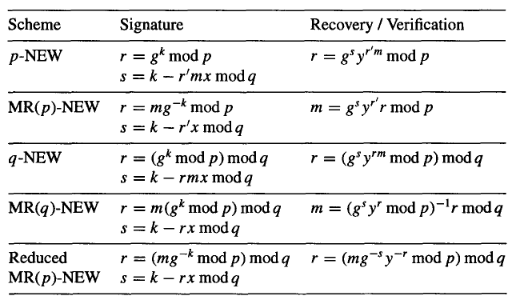
\includegraphics[width=\textwidth]{imagens/nyberg.png}
 
 Todas as variações acima foram geradas à partir do mesmo conjunto
 inicial de equações e por isso são relacionados.
 
 O q-NEW foi o primeiro esquema que mostramos e mostra-se o mais
 atrativo por não precisar de qualquer cálculo de inverso
 multiplicativo. O p-NEW é quase igual, sendo que a principal diferença
 é em qual momento calculamos o módulo $q$ do $r$ ($r'=r \mod q$).
 
 O MR(p)-NEW é a variação que vimos logo depois e que também foi
 apresentada por Ateniese e Medeiros na forma adaptada de um hash
 camaleão.
 
 Podemos mostrar aqui também como seria um hash camaleão baseado na
 forma MR(q)-NEW e Reduced MR(p)-NEW.
 
 O hash camaleão MR(q)-NEW seria:
 
 $$
 Hash(m, (r, s)) = (g^sy^{\mathcal{H}(m||r) \mod p})^{-1}r \mod q
 $$
 $$
 PreImage(c, m) = (c(g^k \mod p) \mod q, k-\mathcal{H}(m||r)x \mod q)
 $$
 
 \textbf{Prova: }Demonstraremos que $Hash(m, PreImage(c, m)) = c$.
 
 \begin{equation*}
 \begin{split}
 &Hash(m, PreImage(c, m))\\
 &= Hash(m, (cg^{k} \mod p, k-x\mathcal{H}(m||r) \mod q))\\
 &= (g^sy^{\mathcal{H}(m||r)})^{-1}r \mod p\\
 &= (g^{s+x\mathcal{H}(m||r)})^{-1}r \mod p\\
 &= (g^{k-x\mathcal{H}(m||r)+x\mathcal{H}(m||r)})^{-1}r \mod p\\
 &= g^{-k}cg^{k} \mod p\\
 &= c\\
 \end{split}
 \end{equation*}
 
 Por fim, o hash camaleão Reduced MR(p)-NEW seria:
 
 $$
 Hash(m, (r, s)) = r-(mg^{-s}y^{-r} \mod p) \mod q
 $$
 
 $$
 PreImage(c, m) = (c+(mg^{-k} \mod p) \mod q, k-rx \mod q)
 $$
 
 \textbf{Prova: }Demonstraremos que $Hash(m, PreImage(c, m)) = c$.
 
 \begin{equation*}
 \begin{split}
 &Hash(m, PreImage(c, m))\\
 &= Hash(m, (c+(mg^{-k} \mod p) \mod q, k-rx \mod q))\\
 &= r-(mg^{-s}y^{-r} \mod p) \mod q\\
 &= r-(mg^{-s-xr} \mod p) \mod q\\
 &= r-(mg^{-k+rx-xr} \mod p) \mod q\\
 &= r-(mg^{-k} \mod p) \mod q\\
 &= c+(mg^{-k} \mod p)-(mg^{-k} \mod p) \mod q\\
 &= c\\
 \end{split}
 \end{equation*}
 
 \subsection{Segurança}
 
 Uma das vantagens de definir hashes camaleão à partir de assinaturas
 digitais é que se as assinaturas são seguras, pode-se derivar deste
 fato muito da segurança das hashes camaleão baseadas nelas.
 
 A resistência à colisão e o fato do esquema ser livre de exposição de
 chave deriva da própria segurança da assinatura de Nyber Rueppel.
 
 Contudo, não necessariamente um esquema de assinatura continua sendo
 seguro se uma mesma mensagem é assinada várias vezes e um atacante tem
 acesso à tais assinaturas. Felizmente, no caso da assinatura de
 Nyberg-Rueppel, isso foi demonstrado em \cite{twin}, no Apêndice A.
 
 Já a segurança semântica deste esquema foi demonstrada por Ateniese e
 Medeiros no artigo que apresentou este esquema de assinatura.
 
 \subsection{Medida de Desempenho}
 
 Este é o desempenho obtido do hash camaleão de Nyberg-Rueppel q-NEW,
 apresentado por Ateniese e Medeiros e que mostra-se mais atrativo por
 não precisar de cálculo de inverso multiplicativo:
 
 \begin{center}
 \begin{tabular}{|c|c|c|c|c|c|}
 \hline
 KeyGen & 0,017544s & Hash & 0,019996s & Collision & 0,007057s\\
 \hline
 \end{tabular}
 \end{center}
 
 \section{Construção Baseada no DSA}
 
 A seção anterior nos leva a questionar se a mesma técnica não poderia
 ser usada para obter hashes camaleão baseados em outras assinaturas
 que também seriam derivadas do Elgamal. Seria uma questão de montar um
 hash à partir da equação de verificação e obter uma função de
 pré-imagem à partir da equação que define a assinatura.
 
 Esta seção mostra que é possível fazer isso com a assinatura DSA.
 
 \subsection{Funções}
 
 \textbf{KeyGen: } A geração de chaves funciona de maneira idêntica à
 geração do DSA. Primeiro escolhe-se dois primos $p$ e $q$ tal que
 $p-1$ é um múltiplo de $q$. Escolhemos então um inteiro $h$ aleatório
 entre 2 e $p-2$. É possível simplesmente usar $h=2$. Por fim,
 computamos $g=h^{(p-1)/q} \mod p$. Assim $(p, q, g)$ são os parâmetros
 de sistema usados pelo algoritmo.
 
 Para a chave privada escolhemos um valor $\mathcal{SK}=x$ menor que
 $q$. E a chave pública é $\mathcal{PK}=y=g^x \mod p$;
 
 \textbf{Hash:}
 
 Verificar uma assinatura DSA $(r, s)$ para uma mensagem $m$ envolve
 checar se é verdade que:
 
 $$
 (g^{\frac{\mathcal{H}(m)}{s} \mod q}y^{\frac{r}{s} \mod q} \mod p) \mod q = r
 $$
 
 Baseando-se nessa equação construímos nossa função de hash:
 
 $$
 Hash(m, (r, s)) = r - (g^{\frac{\mathcal{H}(m)}{s} \mod q}y^{\frac{r}{s} \mod q} \mod p) \mod q
 $$
 
 \textbf{PreImage:}
 
 Criar uma assinatura legítima DSA para a mensagem $m$ envolve escolher
 $(r, s)$ tais que:
 
 $$
 r = (g^k \mod p) \mod q
 $$
 
 $$
 s = k^{-1}(\mathcal{H}(m)+xr) \mod q)
 $$
 
 Exatamente como na primeira assinatura Nyberg-Rueppel da seção
 anteriror, podemos controlar o valor da hash que definimos aqui apenas
 perturbando o valor de $r$ somando à ele o valor do \textit{digest}
 desejado:
 
 $$
 PreImage(m, c) = (c + (g^k \mod p) \mod q,k^{-1}(\mathcal{H}(m)+xr) \mod q)
 $$
 
 \textbf{Prova:}Demonstraremos que $Hash(m, PreImage(c, m)) = c$.
 
 \begin{equation*}
 \begin{split}
 &Hash(m, PreImage(c, m))\\
 &= Hash(m, (c + (g^k \mod p) \mod q, k^{-1}(\mathcal{H}(m)+xr) \mod q))\\
 &= r - (g^{\frac{\mathcal{H}(m)}{s} \mod q}y^{\frac{r}{s} \mod q} \mod p) \mod q\\
 &= r - (g^{\frac{\mathcal{H}(m)+xr}{s} \mod q} \mod p) \mod q\\
 &= r - (g^{\frac{k(\mathcal{H}(m)+xr)}{\mathcal{H}(m)+xr} \mod q} \mod p) \mod q\\
 &= c + (g^k \mod p) - (g^{k} \mod p) \mod q\\
 &= c\\
 \end{split}
 \end{equation*}
 
 \subsection{Segurança}
 
 Assim como na seção anterior, a segurança deste esquema deriva da
 própria segurança do esquema de assinaturas DSA e da propriedade que o
 DSA continua seguro mesmo que um atacante tenha acesso a mais de uma
 assinatura válida para uma mesma mensagem. A segunda propriedade foi
 demonstrada em \cite{twin}.
 
 A segurança semântica deste esquema ainda está para ser demonstrada.
 
 \subsection{Medida de Desempenho}
 
 \begin{center}
 \begin{tabular}{|c|c|c|c|c|c|}
 \hline
 KeyGen & 0,0020026s & Hash & 0,018312s & Collision & 0,006846s\\
 \hline
 \end{tabular}
 \end{center}
 
 
 \section{Construção Baseada no Protocolo Sigma de Fiat-Shamir
 (Mihir Bellare e Todor Ristov) (2008)\cite{sigma}}
 
 Esta construção foi obtida em um artigo no qual os autores estavam
 demonstrando a possibilidade de construir novas funções hash com
 provas de segurança à partir de protocolos sigma. Eles demonstraram
 que as funções hash que eles obtiveram também tinham a propriedade de
 ser hashes camaleão.
 
 \subsection{Funções}
 
 \textbf{KeyGen: } Gere dois primos aleatórios $p$ e $q$. Faça $n=pq$.
 
 Como chave pública, gere um vetor $s$ de $k$ números que sejam
 resíduos quadráticos módulo $n$, sendo $k$ o número de bits das
 mensagens a serem recebidas. Para adotar as melhorias propostas no
 Protocolo Micali-Shamir, tais números devem ser primos pequenos que
 sejam resíduos quadráticos módulo $n$, Adicione também à chave o valor
 $n$.
 
 Como chave privada, gere um vetor $v$ de $k$ números tal que
 $v_i=s_i^{-2} \mod n$ e também adicione à chave os fatores $p$ e $q$.
 
 \textbf{Hash: } Seja a mensagem $m$ um vetor binário com $k$ bits e
 sendo $r \leq n/2$, a hash é obtida por:
 
 $$ Hash(\mathcal{PK}, m, r) = r^2\prod_{m_i=1}v_i \mod n
 $$
 
 \textbf{PreImage: } Esta função é definida como:
 
 $$
 PreImage(\mathcal{SK}, C, m') = \sqrt{C}\prod_{m'_i=1}s_i \mod n
 $$
 
 A raíz quadrada modular só pode ser calculada por quem conheça os
 fatores primos de $n$. A fórmula acima funciona, pois:
 
 $$ C = r^2\prod_{m_i=1}v_i =
 r^2\prod_{m_i=1}\frac{1}{s_i^2}\Longrightarrow r=\sqrt{C}\prod_{m'_i=1}s_i
 $$
 
 \subsection{O Problema da Exposição de Chave}
 
 Esta construção não é livre de exposição de chave. Se somos capazes de
 obter uma colisão na qual as duas mensagens que colidem possuem bits
 1s nas mesmas posições, para cada bit 1 em comum, podemos gerar uma
 nova colisão para novas mensagens idênticas, mas que possuem o bit 1
 correspondente trocado para 0, mantendo os parâmetros aleatórios das
 mensagens idênticos.
 
 Sendo assim, a probabilidade de que uma colisão não revele novas
 colisões derivadas é negligível.
 
 \subsection{Medida de Desempenho}
 
 \begin{center}
 \begin{tabular}{|c|c|c|c|c|c|}
 \hline
 KeyGen & 4,838347s & Hash & 0,000004s & Collision & 0,004199s\\
 \hline
 \end{tabular}
 \end{center}
 
 \section{Construção Baseada no Protocolo Sigma de Okamoto
 (Mihir Bellare e Todor Ristov) (2008)\cite{sigma}}
 
 Esta construção foi obtida assim como a anterior à partir de
 protocolos sigma já existentes após o autor perceber a relação
 existente entre protocolos sigma e hashes camaleão. Mas ao contrário
 do método anterior, esta construção não se destaca por ter vantagem em
 desempenho comparada à outras construções e nem tem a propriedade
 desejável de ser livre de exposição de chave.
 
 \subsection{Funções}
 
 \textbf{KeyGen: } Obtenha um grupo onde calcular o logaritmo discreto
 é um problema difícil. Escolha como chave pública $(g_1, g_2, x)$ onde
 $g_1$ e $g_2$ são geradores e escolha como chave privada $(s_1, s_2)$
 tais que $g_1^{s_1}g_2^{s_2} = x$.
 
 \textbf{Hash: } É definida pela seguinte função:
 
 $$
 Hash(\mathcal{PK}=(g_1, g_2, x), m, r=(r_1, r_2)) = x^mg_1^{r_1}g_2^{r_2}
 $$
 
 \textbf{Collision: } Pela propriedade da exponenciação, dados $m$,
 $m'$ e $r=(r_1, r_2)$ conhecidos, podemos obter $r'=(r_1', r_2')$ tal
 que $Hash(\mathcal{PK}, m, r) = Hash(\mathcal{PK}, m', r')$ por meio
 da equação:
 
 $$
 r_1' = (m-m')s_1+r_1
 $$
 
 $$
 r_2' = (m-m')s_2+r_2
 $$
 
 A mesma equação também nos revela que o esquema não é livre da
 exposição de chaves, pois diante de uma colisão os valores $s_1$,
 $s_2$ podem ser trivialmente isolados.
 
 \textbf{Prova: }Pode-seprovar o funcionamento desta construção
 mostrando que $Hash(m', Collision(m, r, m')) = Hash(m, r)$:
 
 \begin{equation}
 \begin{split}
 Hash(m', Collision(m, r, m'))
 &= Hash(m', ((m-m')s_1+r_1, (m-m')s_2+r_2))\\
 &= x^{m'}g_1^{(m-m')s_1+r_1}g_2^{(m-m')s_2+r_2}\\
 &= x^{m'}x^{m-m'}g_1^{r_1}g_2^{r_2}\\
 &= Hash(m, r)\\
 \end{split}
 \end{equation}
 
 Contudo, embora funcione, este esquema não apresenta qualquer vantagem
 em relação à outros esquemas baseados em logaritmo discreto.
 
 \section{Construction using Lattices (David Cash and Daniele Micciancio)
 (2010 and 2011)\cite{reticulado}\cite{micciancio2012trapdoors}}
 
 This chameleon hash scheme in fact shows how to construct a chameleon
 hash from a regular cryptographic hash function $H$ and a
 probabilistic one-way trapdoor function $f$.
 
 A probabilistic trapdoor function scheme $T$ is a tuple of algorithms
 $(G, F, F^{-1})$ defined over $(X, Y)$. The algorithm $G$ is a
 probabilistic algorithms that givem the security and system
 parameters returns a pair of keys $(\mathcal{PK}_T, \mathcal{SK}_T)$,
 $F$ is a deterministic algorithm that given the security and system
 parameters, the key $\mathcal{PK}$ and $x \in X$, returns $y \in
 Y$. And $F^{-1}$ is a probabilistic algorithm that given the security
 and system parameters, the key $\mathcal{SK}$ and a $y \in Y$,
 returns a $x \in X$ such as $F(x)=y$.
 
 An adversary $\mathcal{A}$ which tries to break the one-way trapdoor
 function security interacts with a challenger which computes:
 $(\mathcal{PK}, \mathcal{SK}) \leftarrow^{\$}G()$, $x
 \leftarrow^{\$}X$, $y \leftarrow^{\$}F(\mathcal{PK}, x)$. The
 challenger sends $y$ to the adversary and the adversary outbuts $\hat
 x \in X$. The adversary wins if $F(\mathcal{PK}, \hat x) = y$. The
 one-way trapdoor function is secure if for all efficient adversaries,
 this probability (represented by OWadv[$\mathcal{A}, T$]) is
 negligible.
 
 The cryptographic hash function $H$ used here will map elements from
 set $A$ to set $Y$. And there's a group defined in the set $Y$ using
 the $+$ operation.
 
 The Cash's chameleon hash scheme is defined over $(A, X, Y)$.
 
This is the Cash's chameleon hash scheme key generation algorithm:

$$
KeyGen() := G()
$$
 
Given the keys taken from the one-way trapdoor function, we define the
$Hash$ algorithm as:

$$
Hash(\mathcal{PK}, m, r) := H(m) - F(\mathcal{PK}, r)
$$

This is a preimage chameleon hash, as we can define the $PreImage$
algorithm as:

$$
PreImage(\mathcal{SK}, m, c) := F^{-1}(\mathcal{SK}, H(m) + c)
$$

\begin{theorem}
The Cash's chameleon hash scheme defined above is a functional
chameleon hash scheme.
\end{theorem}

\textbf{Proof:} We will show that the $r \in R$ obtained by the
$PreImage$ algorithm results in the digest $c$ when used with the
message $m$. Notice that composing $F(\mathcal{PK}, \cdot)$ and
$F^{-1}(\mathcal{SK}, \cdot)$ give us a identity function. The
converse isn't true because $F^{-1}$ is a probabilistic algorithm.

\begin{equation}
 \begin{split}
 Hash(m, r) &= Hash(m, F^{-1}(\mathcal{SK}, H(m) + c))\\
 &= H(m) - F(\mathcal{PK}, F^{-1}(\mathcal{SK}, H(m) + c))\\
&= H(m) - H(m) + c)\\
&= c\\
 \end{split}
 \end{equation} \qed

The main problem with this construction is that not necessarily the
resulting chameleon hash is secure, even if the hash and the one-way
trapdoor function are secure. If we cant't invert the trapdoor
function and can't invert the hash function, we could still compute
$(m, r)$ and $(m', r')$ such as $H(m) - F(\mathcal{PK}, r)=H(m') -
F(\mathcal{PK}, r')$.

When this was originally proposed, wasn't in this general form. The
author suggested using this construction with specific primitives: the
Ajtai Hash Function and a one-way trapdoor function based in lattices.

\subsection{Ajtai's Hash Function}

Given a matrix $A_1$ of integers module $q$ such as $A_1 \in
\mathbb{Z}_q^{m\times n}$, we define the Ajtai hash function defined
over messages $\overrightarrow{m} \in \{0,1\}^{n}$ and digests $t \in
\mathbb{Z}_q^m$ as:

$$
H_A(\overrightarrow{m}) = A\overrightarrow{m} \mod q
$$
 
To understand if this is a secure hash function, let's check what it
means if we can compute the inverse of $H_A$.

For $H_A(\overrightarrow{x})=0$. We know that
$A\overrightarrow{0}=0$. And because $A\overrightarrow{a} + A
\overrightarrow{b} = A(\overrightarrow{a}+\overrightarrow{b})$, we
know that if two vectors are solutions for the equation
$H_A(\overrightarrow{x})=0$, it's sum also is a solution. It means
that the set of all solutions for this equation is in a lattice:

\begin{definicao}
 A \textbf{lattice} is a set of points in $n$-dimentional space with a
 periodic structure. Given $n$ linearlly independent vectors
 $\overrightarrow{b_1},\ldots\overrightarrow{b_n} \in \mathbb{R}^n$
 the lattice generated by them is the set of vectors:
 
 $$
 \mathcal{L}(\overrightarrow{b_1},\ldots\overrightarrow{b_n})=\left\{\sum_{i=1}^nx_i\overrightarrow{b_i}
 : x_i \in \mathbb{Z}\right\}
 $$
 
 The vectors $\overrightarrow{b_1},\ldots\overrightarrow{b_n}$ are the
 \textbf{basis} for the lattice.
\end{definicao}
 
But not all the vectors in the lattice are real solutions for the
equation. By definition, lattices have infinite vectors, but our
number of solutions are clearly finite. As we defined our set of
messages as $\{0, 1\}^n$, only short vectors in the lattice are proper
solutions.

But what if we take the equation
$H_A(\overrightarrow{x})=\overrightarrow{t}$ for some
$\overrightarrow{t}\neq\overrightarrow{0}$? In this case, the vector
$\overrightarrow{0}$ not necessarily is a solution. But we still have
the property that if two vectors are solutions, their sum also is a
solution. In this case, the solution isn't necessarily in a lattice,
but they are in what is called an \textbf{ideal lattice}. We can
convert all ideal lattices to an equivalent lattice summing all their
vectors with a constant in a way that moves one of its points to the
origin.

The problem is that finding short vectors in lattices is believed to
be a very difficult problem. Using known methods, we could compute a
basis for the lattice or ideal lattice, but not a basis with short
vectors. And so, according with the following assumption, we can't do
this except with negligible probability:

\begin{assumption}
\textbf{Short Integer Solution Assumption (SIS$_{n, m, q, \beta}$):
}Given $A \in \mathbb{Z}_q^{n \times m}$ with entries that consists in
$m$ uniformly random vectors as its columns, find a nonzero vector
$\overrightarrow{x} \in \mathbb{Z}^n$ such that:

\begin{itemize}
    \item $||\overrightarrow{x}||\leq \beta < q$
    \item $A\overrightarrow{x}=\overrightarrow{0} \in \mathbb{Z}_q^n$
\end{itemize}

To ensure the existance of nontrivial solutions, is required:

\begin{itemize}
    \item $\beta \geq \sqrt{n\log q}$
    \item $m \geq n \log q$
\end{itemize}

The probability of finding solutions in this problem for any $m, q,
\beta$ is a negligible function over $n$.
\end{assumption}

Given this assumption, we can formulate the following theorem:

\begin{theorem}
  If the SIS assumption is true, then Ajtai's hash function is a
  collision resistant hash function.
\end{theorem}

\textbf{Proof: } For any adversary $\mathcal{A}$ which tries to
compute collisions in Ajtai's hash function, we could create a new
adversary $\mathcal{B}$ which tries to find hort vectors in a lattice.

The adversary $\mathcal{B}$ would take the matrix $A$ and use it to
define an Ajtai's hash function. It would use $\mathcal{A}$ to get a
collision: two values $\overrightarrow{m_1}$ and
$\overrightarrow{m_2}$ such that
$A\overrightarrow{m_1}=A\overrightarrow{m_2}$.

We know that $A(\overrightarrow{m_1}-\overrightarrow{m_2}) =
A\overrightarrow{_m1}-A\overrightarrow{m_2} = 0$, so the adversary
$\mathcal{B}$ can compute $\overrightarrow{m_1}-\overrightarrow{m_2}$
as the answer.

As $\overrightarrow{m_1},\overrightarrow{m_2}\in \{0,1\}^n \subset
\mathbb{Z}_q^n$, then
$||\overrightarrow{_m1}-A\overrightarrow{m_2}||\leq\sqrt{n}<sqrt{n\log
  q \leq \beta}$. The resulting vector is considered a short vector in
the SIS assumption.

The probability of this adversary $\mathcal{B}$ returning a correct
answer is as least as high as the probability of $\mathcal{A}$
returning a collision. So:

$$
\textrm{CRadv}[\mathcal{A}, H_A] \leq Pr[\textrm{Finding\ a\ SIS\ solution}]
$$

As the prbability of solving a SIS problem is negligible by our
hypothesis, then the Ajtai's hash function $H_A$ is collision
resistant. \qed

To ensure that $H_A$ compresses it's input, we neet do set
$|\{0,1\}^m|>|\mathbb{Z}_q^n|$. This condition is always true if $m>n
\log q$ as required to ensure security under the SIS assumption.

If we also want a guarantee that $H_A$ is an one-way function, we need
to ensure that the number of digests without a second-preimage is
negligible. This can be done setting $m$ as $n \log q$ multiplied by
some function of $n$ non-constant and greater than one. For example,
setting $m = n\log n\log q$.


\subsection{Miccianccio One-Way Trapdoor Function}
 
The one-way trapdoor function of this scheme is very similar to the
previous hash function. The $F$ algorithm in the scheme gets a
$\mathcal{PK} = A \in \mathbb{Z}_q^{m \times n}$ and a
$\overrightarrow{x} \in \mathbb{Z}^n$ and $\overrightarrow{x}$ has an
euclidean norm lesser than some small $\beta$ and returns a $y$ such
that:

$$
F(A, \overrightarrow{x}) = y = A\overrightarrow{x} \mod q
$$

This is essentially the same computation that in Ajtai's hash
function. The main difference is that the matrix $A$ here isn't random
and uniform. The majority of columns are, but the last columns hide a
trapdoor.

To understand the trapdoor, notice that while it's difficult to invert
the function $F(A, \cdot)$ for a random and uniform $A$, exist some
matrices for which invert the function is trivial.

Suppose we have matrix $G \in \mathbb{Z}_q^{n \times w}$ for which is
easy to compute $F(A, \cdot)$ and its inverse. Given $G$, we can
construct a family of matrices which could also be inverted reducing
their inversion problem to the inversion of $G$. For example, if we
have:

$$
A\begin{bmatrix}R\\I\end{bmatrix} = G
$$

for $G \in \mathbb{Z}_q^{n \times w}$, a matrix $A \in \mathbb{Z}^{n
  \times m}$, the identity matrix $I \in \mathbb{Z}^{w \times w}$ and
a trapdoor matrix $R \in \mathbb{Z}_q^{(m-w) \times w}$. We can
compute the invrse of $F(A, \overrightarrow{x})$ using this algorithm
if we know the trapdoor $R$ and the inverse of $F(G, \cdot)$:

\begin{equation*}
 \begin{split}
F^{-1}(\mathcal{SK}=(A, R), \overrightarrow{y}) :=& \overrightarrow{p}
\leftarrow^{\$} \mathbb{Z}_q^m\\ &\overrightarrow{v} \leftarrow
\overrightarrow{y} - A\overrightarrow{p} \mod q\\ & \overrightarrow{z}
\leftarrow \textrm{vector\ such\ that\ } F(G,
\overrightarrow{z})=\overrightarrow{v}\\ &\textbf{return\ }\overrightarrow{p}
+ \begin{bmatrix}R\\I\end{bmatrix}\overrightarrow{z}
 \end{split}
 \end{equation*}

 To prove that this works, we just take the value returned by $F^{-1}$
 above, and show that the function $F(A, \cdot)$ maps it to
 $\overrightarrow{y}$ as expected:
 
 \begin{equation*}
 \begin{split}
 F(A, \overrightarrow{p}
 + \begin{bmatrix}R\\I\end{bmatrix}\overrightarrow{z}) &=
   A(\overrightarrow{p}
   + \begin{bmatrix}R\\I\end{bmatrix}\overrightarrow{z})\\ &=
     A\overrightarrow{p} +
     A\begin{bmatrix}R\\I\end{bmatrix}\overrightarrow{z}\\ &=
     A\overrightarrow{p} + G\overrightarrow{z}\\
 \end{split}
 \end{equation*}
 
 But we know that
 $G\overrightarrow{z}=\overrightarrow{z}=\overrightarrow{y} -
 A\overrightarrow{p}$:
 
  \begin{equation*}
 \begin{split}
 F(A, \overrightarrow{p}
 + \begin{bmatrix}R\\I\end{bmatrix}\overrightarrow{z}) &=
   A\overrightarrow{p} + \overrightarrow{y} - A\overrightarrow{p}\\ &=
   \overrightarrow{y}\\
  \end{split}
 \end{equation*}
 
 But the value $\overrightarrow{x}$ generated by $F^{-1}$ also need to
 be a small value. To ensure this, the random vector
 $\overrightarrow{p}$ generated in the first line of $F^{-1}$ must be
 a small vector and the trapdoor $R$ must be a matrix with small
 values. When they are small enough, $\overrightarrow{p}
 + \begin{bmatrix}R\\I\end{bmatrix}\overrightarrow{z}$ also will be a
   small vector with high probability. If not, we could try again
   choosing a different probabilistic $\overrightarrow{p}$.
 
 \subsubsection{Choosing G}
 
 In an exemple of $n=2$ and $q=8$ or some other power of two, we could
 choose the following $G$:
 
 $$ G = \begin{bmatrix}1 & 2 & 4 & 0 & 0 & 0\\0 & 0 & 0 & 1 & 2&
   4\end{bmatrix}
 $$
 
 If we want to discover a value $\overrightarrow{x}$ such that
 $G\overrightarrow{x}=\overrightarrow{y}$, we could find it choosing
 $\overrightarrow{x}$ as the binary representation of
 $\overrightarrow{y}$. For example, if
 $\overrightarrow{y}=\begin{bmatrix}5\\2\end{bmatrix}$, then
 $\overrightarrow{x}=\begin{bmatrix}1&0&1&0&1&0\end{bmatrix}^T$.
 
 For bigger values of $n$ and $q$, we just use bigger matrices $G$
 built with this method. But instead of using the simpler binary
 representation above, we can get better results using algorithms of
 gaussian sampling over lattices.
 
 \subsubsection{Choosing the Matrix A and the One-Way Trapdoor
   Function Security}

 We want to choose a matrix $A \in \mathbb{Z}_q^{n \times m}$ such
 that $A\begin{bmatrix}R\\I\end{bmatrix} = G$.
 
 We can choose then:
 
 $$
 A = \begin{bmatrix}\overline{A} & G-\overline{A}R\end{bmatrix}
 $$
 
 when $\overline{A} \in \mathbb{Z}_q^{n \times (m-w)}$ is a random uniform matrix.
 
\begin{theorem}
 The Micciancio's one-way trapdoor scheme $I$ is secure if Ajtai's
 hash function $H_A$ is also an one-way function.
\end{theorem}
 
\textbf{Proof: }For all adversaries $\mathcal{A}$ which try to invert
Micciancio's one-way function, we could build a new adversary
$\mathcal{B}$ which try to invert Ajtai's hash function.

Adversary $\mathcal{B}$ gets matrix $A$ as a system parameter. Then it
sets $\overline{A}=A$, chooses a trapdoor $R$ and sends to adversary
$\mathcal{A}$ the public key $\begin{bmatrix}\overline{A} &
  G-\overline{A}R\end{bmatrix}$.

Adversary $\mathcal{B}$ gets from its challenger a digest
$\overrightarrow{t_1} \in \mathbb{Z}_q^n$ such that
$\overrightarrow{t_1}=A\overrightarrow{x} \mod q$. It chooses a random
$\overrightarrow{m*} \in \mathbb{Z}_q^{w}$ where $w$ is the number of
columns of $G$. It computes $\overrightarrow{t_2} =
(G-\overline{A}R)\overrightarrow{m*}$. Finally, it sends
$\overrightarrow{t_1}+\overrightarrow{t_2}$ as the challenge to
adversary $\mathcal{A}$ and gets the answer $\overrightarrow{m}$.

Let $\overrightarrow{m}=\overrightarrow{m_1}||\overrightarrow{m_2}$
with $m_1 \in \mathbb{Z}_q^m$. Adversary $\mathcal{B}$ returns
$\overrightarrow{m_1}$.

If $\mathcal{A}$ outputs a correct answer, it means that
$\overline{A}\overrightarrow{m_1} +
(G-\overline{A}R)\overrightarrow{m_2}=\overrightarrow{t_1} +
\overrightarrow{t_2}$. Notice that if $m_2=m*$, then
$\overline{A}\overrightarrow{m_1}=\overrightarrow{t_1}$ and so
$\overrightarrow{m_1}=\overrightarrow{x}$. So we have:

$$ \textrm{OWadv}[\mathcal{B},H_B] \geq \textrm{OWadv}[\mathcal{A},
  I]\cdot Pr[\overrightarrow{m_2}=\overrightarrow{m*}]
$$

If $\mathcal{A}$ returned a correct answer, it means that $m_2$ always
will be a correct solution to the system of equations represented by
$(G-\overline{A}R)\overrightarrow{m_2} =
\overrightarrow{t_1}+\overrightarrow{t_2} -
\overline{A}\overrightarrow{m_1}$. As $G \in \mathbb{Z}_q^{n \times
  w}$, the number of solutions is bounded by $w-n+1$. For the specific
$G$ presented in this section, $w=n\log q$.

We can combine these results and get:

$$ \textrm{OWadv}[\mathcal{A},I] \leq n\log q \cdot
\textrm{OWadv}[\mathcal{B}, A_H]
$$

This completes the proof that if Ajtai's hash function $H_A$ is an
one-way function, Micciancio's one-way trapdoor function is
secure. \qed


\subsection{Combining the Constructions to Create the Chameleon Hash}

\subsubsection{Security and System Parameters}

The security parameter $\lambda$ here means the number of lines in the
matrices for Ajtai's hash function and Micciancio's one-way trapdoor
function.

Ajtai's hash matrix will be a fixed random and unifrom $n \times m$
matrix $A_1$ modulo $q$ which could be the same matrix in all
implementations with $m \geq n \log q$. And $q$ is some fixed value
chosen to be convenient. It could be some power of two which could
represent the numbers which could be stored in 32 or 64 bits. Both
$A_1$ and $q$ are encoded in system paramenter $\Lambda$.

\subsubsection{Key Generation}

The key generator algorithm should generate the one-way trapdoor function's public and private keys. The public key is a matrix $A_2=\begin{bmatrix}\overline{A} & G-\overline{A}R\end{bmatrix}$

The private key is the trapdoor matrix $R$. Assuming that we use as $G$ the power-of-two matrix seen in the last section, $G \in \mathbb{Z}_q^{n \times n \log q}$. So $R$ need to have $n \log q$ columns. The number of lines in $R$ depends of the number of columns in the matrix $\overline{A}$. To ensure the same degree of security, we choose the same $m \geq n \log q$ used in the matrix $A_1$ from Ajtai's hash function. So $R\in \mathbb{Z}_q^{m \times n \log q}$.

Given the trapdoor $R$, we can compute a random and uniform $\overline{A}\in \mathbb{Z}_q^{n \times m}$. And from this we compute $A_2\in\mathbb{Z}_q^{n \times mn \log q}$.

The public key is $\mathcal{PK}=A_2$ and the private key is $\mathcal{SK}=(A_2, R)$.

As these matrices could be very large, more realistically we could generate these matrices using some pseudo-random generator $G$ and smaller keys. We could generate $\overline{A}$ from some key $k_1$ and $R$ from other key $k_2$. Our private key would be $\mathcal{SK}=(k_1, k_2)$. Unfortunally this compresses just the first $m$ columns of the matrix $A_2$. The last $n \log q$ columns hide our trapdoor and can't be easily compressed. So our public key would be $\mathcal{PK}=(k_1, G-\overline{A}R)$, meaning that we still need to store a matrix with $n^2\log q$ elements in the public key.




 \bibliography{report}{}\bibliographystyle{plain}
 \end{document}
 %%%%%%%%%%%%%%%%%%%%%%%%%%%%%%%%%%%%%%%%%%%%%%%%%%%%%%%%%%%%%%%%%
 
 \section{Hashes Camaleão com ID}
 
 \subsection{Construção Baseada no RSA (Ateniese e Medeiros) (2005)\cite{ateniese2004key}}
 
 Este esquema se baseia nas propriedades da assinatura e criptografia
 RSA. Elas nos dizem que se temos dois primos grandes $p$ e $q$,
 podemos obter um número primo em relação a $\phi(pq)$ que chamamos de
 $e$ e o seu inverso multiplicativo módulo $\phi(pq)$, que chamamos de
 $d$. Seja $n=pq$.
 
 Temos então que $M'=M^e \mod n$ e $M=M'^d \mod n$. Tratamos $(e, n)$
 como a chave pública e $(d, p, q)$ como a chave privada. As chaves
 podem ser calculadas facilmente somente por alguém que conhece os
 fatores primos que formam $n$.
 
 \subsection{Funções}
 
 \textbf{KeyGen: } Idêntica à geração de chaves do RSA. A chave pública
 é $(e, n)$ e a chave privada é $(d, p, q)$. A única restrição
 adicional é que $e$ deve ser um número primo, não apenas primo em
 relação a $\phi(n)$.
 
 \textbf{Hash: } Assuma que esta função além da mensagem $m$ e do
 parâmetro $r$ recebe também um $\mathcal{L}$ que representa uma
 identificação ou rótulo da operação sendo realizada. Seja $C$ e
 $\mathcal{H}$ duas funções hash convencionais com um tamanho ajustado
 de acordo com parâmetros de segurança e de modo que $\mathcal{H}$ gere
 valores sempre menores que $e$.
 
 Calculamos o hash camaleão calculandoda seguinte forma:
 
 $$
 Hash(\mathcal{L}, m, r) = C(\mathcal{L})^{\mathcal{H}(m)}r^e \mod n
 $$
 
 \textbf{PreImage:} Não está presente neste esquema.
 
 \textbf{UForge:} Para obtermos um novo valor $r'$ para um dado $m'$
 que tenha mesmo hash que $m$ e $r$, podemos comaçar pela equação:
 
 $$
 C(\mathcal{L})^{\mathcal{H}(m)}r^e \equiv C(\mathcal{L})^{\mathcal{H}(m')}r'^e \pmod n
 $$
 
 Dividindo ambos os lados da equação por $C(\mathcal{L})^{\mathcal{H}(m')}$:
 
 $$
 C(\mathcal{L})^{\mathcal{H}(m)-\mathcal{H}(m')}r^e \equiv r'^e \pmod n
 $$
 
 Fazendo a equação ser elevada ao expoente $d$ (que pertence à chave
 privada):
 
 $$
 rC(\mathcal{L})^{d(\mathcal{H}(m)-\mathcal{H}(m'))} \equiv r' \pmod n
 $$
 
 E portanto, podemos calcular $r'$ por meio de \textbf{UForge} com a
 equação abaixo:
 
 $$
 r' = rC(\mathcal{L})^{d(\mathcal{H}(m)-\mathcal{H}(m'))} \mod n
 $$
 
 \textbf{iForge:} É possível extrair o valor $C(\mathcal{L})^d$ por
 meio de uma colisão, que representa uma assinatura RSA sobre o valor
 $\mathcal{L}$. Obtendo este valor, pode-se criar qualquer outra
 colisão neste esquema de hash, mesmo sem sermos capazes de obter a
 chave privada $d$.
 
 O modo de obter $C(\mathcal{L})^d$ é à partir das equações
 acima. Temos inicialmente que:
 
 $$
 r'/r \equiv C(\mathcal{L})^{d(\mathcal{H}(m)-\mathcal{H}(m'))} \pmod n
 $$
 
 Como $e$ é primo e maior que qualquer valor retornado por
 $\mathcal{H}$, então $mdc(e, \mathcal{H}(m)-\mathcal{H}(m')) = 1$. E
 portanto, usando o Algoritmo Estendido de Euclides, podemos obter
 valores $\alpha$ e $\beta$ tais que
 $\alpha(\mathcal{H}(m)-\mathcal{H}(m'))+\beta e = 1$.
 
 Elevando os dois lados da equação acima por $\alpha$ ficamos com:
 
 $$
 (r'/r)^\alpha \equiv C(\mathcal{L})^{d(\mathcal{H}(m)-\mathcal{H}(m'))\alpha} \pmod n
 $$
 
 E multiplicando por $C(\mathcal{L})^{d\beta e}$:
 
 $$
 (r'/r)^\alpha C(\mathcal{L})^{d\beta e} \equiv C(\mathcal{L})^{d(\mathcal{H}(m)-\mathcal{H}(m'))\alpha + d\beta e} \pmod n
 $$
 
 Pela propriedade do RSA, elevar um valor à $d$ e depois à $e$ temos a
 identidade do valor no lado esquerdo da equação. E pela propriedade de
 $\alpha$ e $\beta$ que escolhemos, no lado direito da equação podemos
 simplificar a combinação linear destes valores no expoente por
 1. Portanto extraímos assim o valor que queríamos:
 
 $$
 (r'/r)^\alpha C(\mathcal{L})^{\beta} \mod n= C(\mathcal{L})^d
 $$
 
 \subsection{Propriedades}
 
 \textbf{Resistência a Colisão: }Sim, assumindo que não é possível
 forjar uma assinatura RSA, que o valor de $\mathcal{L}$ nunca foi
 utilizado antes de modo que alguma colisão tenha sido obtida e que as
 funções hash $C$ e $\mathcal{H}$ atendem às propriedades esperadas de
 hashes criptográficas.
 
 \textbf{Ocultação de Mensagem: }Sim, pois foi definida uma função
 \textbf{IForge}.
 
 \textbf{Livre de Exposição de Chave: } Sim. Expor uma colisão não
 expõe a chave privada, apenas uma assinatura RSA sobre $\mathcal{L}$,
 o qual assumimos que é um valor único que não é reaproveitado.
 
 \textbf{Cálculo de Primeira Pré-Imagem: }Não.
 
 \subsection{Construção Baseada em Assinatura Boneh-Lynn-Shacham (Zhang) \cite{zhang}}
 
 Seja $G_1$ e $G_2$ dois grupos (cuja operação será escrita aqui na
 notação multiplicativa) nos quais dado um gerador $g$ e valores $g^x$
 e $g^y$, é difícil computar $g^{xy}$ (Problema Computacional
 Diffie-Hellman). E seja $e$ uma função que associa dois elementos do
 primeiro grupo a um elemento do segundo tal que $e(g^a, g^b) = e(g,
 g)^{ab}$ e $e(g, g) \neq 1$.
 
 Qundo temos um grupo onde tais operações existem, temos um grupo de
 Lacuna Diffie-Hellman, onde é difícil resolver o Problema
 Computacional Diffie-Hellman descrito acima, mas onde é fácil de
 resolver sua variante de decisão, o Problema de Decisão
 Diffie-Hellman. Ele consiste em responder se dados quatro valores
 pertencentes a um grupo ($g$, $g^x$, $g^y$ e $G^z$) temos que $xy=z$.
 
 Resolver tal problema de decisão torna-se fácil em tais grupos porque
 isso é equivalente a responder se $e(g, g^z) = e(g^x, g^y)$.
 
 Como consequência de sua definição, a função de emparelhamento
 bilinear tem também as seguintes propriedades:
 
 \begin{itemize}
 \item$e(pr, q) = e(p, q)e(r, q)$
 \item$e(a^b, c) = e(a, c^b)$
 \end{itemize}
 
 As duas propriedades acima e a dificuldade do Problema Computacional
 Diffie-Hellman é o que garante que a construção desta seção funcione.
 
 \subsection{Funções}
 
 \textbf{KeyGen: }Dado um grupo multiplicativo que é um grupo de Lacuna
 Diffie-Hellman, escolha um valor inteiro $s$ como chave privada e um
 valor $g^s$ pertencente ao grupo como chave pública.
 
 \textbf{Hash: } Assim como no esquema anterior, assuma que a função de
 hash recebe um parâmetro único $\mathcal{L}$ e que existem duas
 funções hash criptográficas comuns que são usadas: $C$ e
 $\mathcal{H}$.
 
 O hash camaleão é calculado pela fórmula:
 
 $$
 Hash(\mathcal{L}, m, r) = e(r, g)e(C(m)^{\mathcal{H}(\mathcal{L})}, g^s)
 $$
 
 \textbf{PreImage:} Não está presente neste esquema.
 
 \textbf{UForge:} Para obtermos um novo valor $r'$ para um dado $m'$
 que tenha mesmo hash que $m$ e $r$ e quando conhecemos a chave privada
 $s$ é obtido pela fórmula:
 
 $$
 UForge(\mathcal{L}, s, m, r, m') = \left[\frac{C(m)}{C(m')}^{\mathcal{H}(\mathcal{L})^s}\right]r = r'
 $$
 
 Isso funciona pois se formos calcular o hash de $m'$ com este $r'$
 calculado, o resultado será:
 
 \begin{equation}
 \begin{split}
 Hash(\mathcal{L}, m', r') &= e(r', g)e(C(m')^{\mathcal{H}(\mathcal{L})}, g^s)\\
 &= e(\left[\frac{C(m)}{C(m')}^{\mathcal{H}(\mathcal{L})^s}\right]r, g)e(C(m')^{\mathcal{H}(\mathcal{L})}, g^s)\\
 &=e(\left[\frac{C(m)}{C(m')}^{\mathcal{H}(\mathcal{L})^s}\right], g)e(r, g)e(C(m')^{\mathcal{H}(\mathcal{L})}, g^s)\\
 &=e(\left[\frac{C(m)}{C(m')}^{\mathcal{H}(\mathcal{L})}\right], g^s)e(r, g)e(C(m')^{\mathcal{H}(\mathcal{L})}, g^s)\\
 &=e(C(m)^{\mathcal{H}(\mathcal{L})}, g^s)e(r, g)\\
 &= Hash(\mathcal{L}, m, r)\\
 \end{split}
 \end{equation}
 
 \textbf{IForge:} Não está definida neste esquema. Poderia ser feito se
 uma forma de isolar $\mathcal{H}(\mathcal{L})^s$ à partir de uma
 colisão fôsse encontrada.
 
 \subsection{Propriedades}
 
 \textbf{Resistência a Colisão: }Sim se assumirmos que é difícil forjar
 um esquema de assinatura Boneh–Lynn–Shacham e que o valor
 $\mathcal{L}$ não é reaproveitado em diferentes hashes camaleão.
 
 \textbf{Ocultação de Mensagem: }Não, pois uma função \textbf{IForge}
 não foi definida.
 
 \textbf{Livre de Exposição de Chave: } Sim.
 
 \textbf{Cálculo de Primeira Pré-Imagem: }Não.
 
 \subsection{Construção Baseada em Emparelhamento Bilinear (Zhang) \cite{zhang}}
 
 Este esquema é proposto no mesmo artigo que o anterior e é uma forma
 alternativa de construir hash camaleão com emparelhamnento bilinear.
 
 \subsection{Funções}
 
 \textbf{KeyGen: }Exatamente como no esquema anterior, dado um grupo
 multiplicativo que é um grupo de Lacuna Diffie-Hellman, escolha um
 valor inteiro $s$ como chave privada e um valor $g^s$ pertencente ao
 grupo como chave pública.
 
 \textbf{Hash: } Aqui o método de cálculo da hash se dá pela fórmula:
 
 $$
 Hash(\mathcal{PK}=g^s, \mathcal{L}, m, r) = e(g, g^{\mathcal{H}(m)})e(g^{\mathcal{H}(\mathcal{L})}g^s, r)^{\mathcal{H}(m)}
 $$
 
 \textbf{PreImage:} Não. Assim como no caso anterior, seria
 necessário resolver o problema do logaritmo discreto para implementar
 esta função.
 
 \textbf{UForge:} Para obtermos um novo valor $r'$ para um dado $m'$
 que tenha mesmo hash que $m$ e $r$ e quando conhecemos a chave privada
 $s$, aproveitamos as seguintes fórmulas:
 
 $$
 S_{ID} = g^{\frac{1}{s+\mathcal{H}(\mathcal{L})}}
 $$
 
 $$
 UForge(\mathcal{SK}=s, \mathcal{L}, m, r, m') = S_{ID}^{\mathcal{H}(m)-\mathcal{H}(m')^{\mathcal{H}(m')}}r^{\mathcal{H}(m)^{-1}} = r'
 $$
 
 Isso funciona pois se formos calcular o hash de $m'$ com este $r'$
 calculado, o resultado será:
 
 \begin{equation}
 \begin{split}
 Hash(\mathcal{PK},\mathcal{L}, m', r') &= e(g, g)^{\mathcal{H}(m')}e(g^{\mathcal{H}(\mathcal{L})}g^s, r')^{\mathcal{H}(m')}\\
 &= e(g, g)^{\mathcal{H}(m')}e(g^{\mathcal{H}(\mathcal{L})}g^s, S_{ID}^{\mathcal{H}(m)-\mathcal{H}(m')^{\mathcal{H}(m')^{-1}}}r^{\mathcal{H}(m)})^{\mathcal{H}(m')}\\
 &= e(g, g)^{\mathcal{H}(m')}e(g^{\mathcal{H}(\mathcal{L})}g^s, S_{ID}^{\mathcal{H}(m)-\mathcal{H}(m')}r^{\mathcal{H}(m)})\\
 &= e(g, g^{\mathcal{H}(m')})e(g^{\mathcal{H}(\mathcal{L})}g^s, g^{\frac{\mathcal{H}(m)-\mathcal{H}(m')}{s+\mathcal{H}(\mathcal{L})}}r^{\mathcal{H}(m)})\\
 &= e(g, g^{\mathcal{H}(m')})e(g^{\mathcal{H}(\mathcal{L})}g^s, g^{\frac{\mathcal{H}(m)-\mathcal{H}(m')}{s+\mathcal{H}(\mathcal{L})}})e(g^{\mathcal{H}(\mathcal{L})}g^s, r^{\mathcal{H}(m)})\\
 &= e(g, g^{\mathcal{H}(m')})e(g, g^{\mathcal{H}(m)-\mathcal{H}(m')})e(g^{\mathcal{H}(\mathcal{L})}g^s, r^{\mathcal{H}(m)})\\
 &= e(g, g^{\mathcal{H}(m')}g^{\mathcal{H}(m)-\mathcal{H}(m')})e(g^{\mathcal{H}(\mathcal{L})}g^s, r^{\mathcal{H}(m)})\\
 &= e(g, g)^{\mathcal{H}(m)}e(g^{\mathcal{H}(\mathcal{L})}g^s, r)^{\mathcal{H}(m)}\\
 &= Hash(\mathcal{PK},\mathcal{L}, m, r)
 \end{split}
 \end{equation}
 
 \textbf{IForge:} Não está definida neste esquema. Poderia ser feito se
 uma forma de isolar $S_{ID} =
 g^{\frac{1}{s+\mathcal{H}(\mathcal{L})}}$ à partir de uma colisão
 fôsse encontrada.
 
 \subsection{Propriedades}
 
 \textbf{Resistência a Colisão: }Sim se assumirmos que é difícil
 calcular o logaritmo discreto e obter o valor $s$ da chave privada e
 que $\mathcal{L}$ não é reaproveitado em diferentes hashes camaleão.
 
 \textbf{Ocultação de Mensagem: }Não, pois uma função \textbf{IForge}
 não foi definida.
 
 \textbf{Livre de Exposição de Chave: } Sim.
 
 \textbf{Cálculo de Primeira Pré-Imagem: }Não.
 
 \subsection{Construção Baseada em Logaritmo Discreto de Chen (Chen)
 \cite{chen}}
 
 O primeiro método baseado em logaritmo discreto proposto por Krawczyk
 tinha o grave problema de exposição de chaves. Este método foi criado
 precisamente para ser livre deste problema. Assim como o método
 anterior, ele requer que utilizemos um Grupo de Lacuna
 Diffie-Hellman. Nas construções anteriores, a principal vantagem de se
 utilizar tal grupo estava mais nas propriedades convenientes da função
 de emparelhamento bilinear. Neste método, o objetivo de usar tais
 grupos está realmente em explorar a vantagem de resolver o Problema de
 Decisão Diffie-Hellman como um teste de sanidade para o valor de $r$.
 
 \subsection{Funções}
 
 \textbf{KeyGen: }A chave pública é um valor $y=g^x$ senfo $g$ um
 gerador. A chave privada é o valor $x$.
 
 \textbf{Hash: }Neste esquema, podemos considerar o valor de $r$ como
 sendo uma tupla na seguinte forma:
 
 $$
 r = (g^a, y^a)
 $$
 
 Com ele calculamos o hash camaleão de acordo com a fórmula:
 
 $$
 Hash(\mathcal{PK}=y, \mathcal{L}, m, r) = (g\mathcal{L})^my^a
 $$
 
 Notar que o primeiro valor da tupla não é usado diretamente no cálculo
 da hash. Ele é usado para checar se realmente temos um valor de $r$
 válido que deve ser aceito. Para isso, basta verificarmos se $g$, $y$,
 $g^a$ e $y^a$ formam uma Tupla Diffie-Hellman ($(\lg y)(\lg g^a) =(\lg
 y^a)$).
 
 \textbf{PreImage:} Não definida.
 
 \textbf{UForge:} Sendo o valor de $r$ uma tupla, ela pode ser obtida
 com:
 
 $$UForge(\mathcal{SK}=x, \mathcal{L}, m, r=(g^a,y^a), m') =
 \big(g^a(g\mathcal{L})^{\frac{m-m'}{x}}, y^a(g\mathcal{L})^{m-m'}\big) =
 (g^{a'}, y^{a'}) = r'
 $$
 
 Pode-se verificar que este valor é o correto, pois se o usarmos para o
 cálculo de uma hash obteremos:
 
 \begin{equation}
 \begin{split}
 Hash(\mathcal{PK},\mathcal{L}, m', r') &= (g\mathcal{L})^{m'}y^{a'}\\
 &= (g\mathcal{L})^{m'}y^{a}(g\mathcal{L})^{m-m'}\\
 &= (g\mathcal{L})^{m}y^{a}\\
 &= Hash(\mathcal{PK},\mathcal{L}, m, r)\\
 \end{split}
 \end{equation}
 
 \textbf{IForge:} Tendo-se uma colisão, podemos extrair o valor $T =
 (g\mathcal{L})^{x^{-1}}$ graças ao primeiro valor da tupla $r$ e $r'$:
 
 $$
 T = (g\mathcal{L})^{x^{-1}} = \left(\frac{g^a}{g^{a'}}\right)^{(m-m')^{-1}}
 $$
 
 Com este valor, pode-se obter uma função \textbf{IForge} escolhendo
 qualquer valor $m''$ e à partir dele calculando um novo $r''$:
 
 $$ IForge(\mathcal{PK}=g^x, \mathcal{L}, m, r=(g^a, y^a), m',
 r'=(g^{a'}, y^{a'})) = (m'', r''=(g^aT^{m-m''},
 y^{a}(g\mathcal{L})^{m-m''}))
 $$
 
 Isso também pode ser usado para demonstrar a segurança deste
 esquema. No artigo em que ele é proposto, prova-se que obter um valor
 $g^{a^{-1}}$ dado $g$ e $g^a$ é tão difícil quanto resolver o Problema
 Computacional Diffie-Hellman. Sendo assim, encontrar uma colisão sem o
 uso da chave privada neste esquema é também tão difícil quanto
 resolver uma instância do Problema Computacional Diffie-Hellman.
 
 \subsection{Propriedades}
 
 \textbf{Resistência a Colisão: }Sim se assumirmos que é difícil resolver o Problema COmputacional Diffie-Hellman.
 
 \textbf{Ocultação de Mensagem: }Sim.
 
 \textbf{Livre de Exposição de Chave: } Sim.
 
 \textbf{Cálculo de Primeira Pré-Imagem: }Não.
 
 \section{Construção Baseada em Diffie-Hellman \cite{ateniese2004key}}
 
 \subsection{Funções}
 
 \textbf{KeyGen: }Em um grupo que é de Lacuna Diffie-Hellman, escolha
 um gerador $g$ e como chave pública um elemento $y=g^x$, sendo o
 inteiro $x$ a chave privada.
 
 \textbf{Hash: }Use a seguinte função para o cálculo de hash:
 
 $$
 Hash(\mathcal{L}, m, r) = g^{\mathcal{H}(m)}(g^{\mathcal{H}(\mathcal{L})}y)^r
 $$
 
 O valor pode ser conferido rapidamente observando que $(g^r,
 yg^{\mathcal{H}(\mathcal{L})}, Hash(\mathcal{L}, m,
 r)/g^{\mathcal{H}(m)})$ é uma Tripla Diffie-Hellman.
 
 \textbf{PreImage:} Não definida.
 
 \textbf{UForge:} A pode ser obtida baseando-se na seguinte equação:
 
 $$
 g^{r'}=g^rg^{\frac{\mathcal{H}(m)-\mathcal{H}(m')}{x+\mathcal{H}(\mathcal{L})}}
 $$
 
 E isso permite obter o valor $r'$ desejado:
 
 $$
 UForge(\mathcal{SK}=x, \mathcal{L}, m, r, m') = r + \frac{\mathcal{H}(m)-\mathcal{H}(m')}{x+\mathcal{H}(\mathcal{L})} = r'
 $$
 
 Isso funciona, pois:
 
 \begin{equation}
 \begin{split}
 Hash(\mathcal{L}, m', r') &= g^{\mathcal{H}(m')}(g^{\mathcal{H}(\mathcal{L})}y)^{r'}\\
 &=g^{\mathcal{H}(m')}(g^{\mathcal{H}(\mathcal{L})}y)^{r + \frac{\mathcal{H}(m)-\mathcal{H}(m')}{x+\mathcal{H}(\mathcal{L})}}\\
 &=g^{\mathcal{H}(m')}(g^{\mathcal{H}(\mathcal{L})}y)^{r}(g^{\mathcal{H}(\mathcal{L})}y)^{\frac{\mathcal{H}(m)-\mathcal{H}(m')}{x+\mathcal{H}(\mathcal{L})}}\\
 &=g^{\mathcal{H}(m')}(g^{\mathcal{H}(\mathcal{L})}g^x)^{r}(g^{\mathcal{H}(\mathcal{L})}g^x)^{\frac{\mathcal{H}(m)-\mathcal{H}(m')}{x+\mathcal{H}(\mathcal{L})}}\\
 &=g^{\mathcal{H}(m')}(g^{\mathcal{H}(\mathcal{L})}g^x)^{r}g^{\frac{(x+\mathcal{H}(\mathcal{L}))(\mathcal{H}(m)-\mathcal{H}(m'))}{x+\mathcal{H}(\mathcal{L})}}\\
 &=g^{\mathcal{H}(m')}(g^{\mathcal{H}(\mathcal{L})}g^x)^{r}g^{\mathcal{H}(m)-\mathcal{H}(m')}\\
 &=g^{\mathcal{H}(m)}(g^{\mathcal{H}(\mathcal{L})}g^x)^{r}\\
 &=g^{\mathcal{H}(m)}(g^{\mathcal{H}(\mathcal{L})}y)^{r}\\
 &=Hash(\mathcal{L}, m, r)\\
 \end{split}
 \end{equation}
 
 \textbf{IForge:} Tendo-se acesso à uma colisão, pode-se usar as
 fórmulas anteriores para extrair o valor
 $g^{\frac{1}{x+\mathcal{H}(m)}}$:
 
 $$
 \left(\frac{g^{r'}}{g^r}\right)^{[\mathcal{H}(m)-\mathcal{H}(m')]^{-1}} = g^{\frac{1}{x+\mathcal{H}(m)}}
 $$
 
 
 Com este valor, mesmo sem conhecermos o valor de $x$ podemos calcular
 um valor correspondente de $r''$ para qualquer novo $m''$ sem
 precisarmos conhecer a chave privada $x$.
 
 \subsection{Propriedades}
 
 \textbf{Resistência a Colisão: }Sim. O artigo que propõe o esquema
 argumenta que mesmo quando conhecemos vários valores diferentes para
 $g^{\frac{1}{x+\mathcal{H}(m)}}$ em diferentes valores de
 $\mathcal{L}$ isso não enfraquece o esquema, usando como referência
 algo demonstrado em outro artigo.
 
 \textbf{Ocultação de Mensagem: }Sim.
 
 \textbf{Livre de Exposição de Chave: }Sim.
 
 \textbf{Cálculo de Primeira Pré-Imagem: }Não.
 
 \section{Construção Baseada em Criptossistema de Pallier (Ateniese e Medeiros) \cite{ateniese2004key}}
 
 Essa construção se baseia na propriedade demonstrada por
 Paillier\cite{paillier} de que a função abaixo, para qualquer $h \in
 \mathbb{Z}^*_{n^2}$, $a\in\mathbb{Z}_n$, $b\in\mathbb{Z}^*_{n^2}$ é
 uma função de permutação com trapdoor:
 
 $$
 f(a, b) = h^aqb^n \mod n^2
 $$
 
 Ou seja, ela pode ser invertida por qualquer um que conheça um segredo
 associado à função (no caso, os fatores de $n$) e além disso ela é uma
 função de permutação.
 
 \subsection{Funções}
 
 \textbf{KeyGen: } Escolha dois primos grandes $p$ e $q$ como chave
 privada. E a multiplicação deles $n=pq$ é a chave pública.
 
 \textbf{Hash: } Assumindo que $\mathcal{H}$ é uma função hash
 criptográfica que tem como codomínio valores em $\mathbb{Z}^*_{n^2}$,
 que o nossa mensagem $m$ foi previamente transformada por alguma
 função hash com codomínio em $\mathbb{Z}^*_{n}$ e que $r = (r_1,
 r_2)$, nossa função de hash camaleão é:
 
 $$
 Hash(\mathcal{L}, m, (r_1, r_2)) = (1 +mn)\mathcal{H}(\mathcal{L})^{r_1}r_2^n \pmod{n^2}
 $$
 
 \textbf{PreImage:} Essa função torna-se possível graças à função
 de permutação com trapdoor ($f$) associada aos criptossistemas de
 Paillier. Primeiro escolhemos a função $f$ específica para
 $h=\mathcal{H}(\mathcal{L})$. Com ajuda dela, obtemos a primeira
 pré-imagem da seguinte maneira:
 
 $$
 PreImage(\mathcal{SK}, m', C) = f^{-1}(C(1-m'n)) = (r_1', r_2')
 $$
 
 Isso funciona, pois geramos valores $r_1'$ e $r_2'$ tais que:
 
 \begin{equation}
 \begin{split}
 f(r_1', r_2') &= C(1-m'n)\\
 \mathcal{H}(\mathcal{L})^{r_1'}r_2'^n &\equiv C(1-m'n) \pmod{n^2}\\
 \end{split}
 \end{equation}
 
 Então se passarmos os valores $m'$, $r_1'$ e $r_2'$ para a função de
 hash camaleão, obtemos:
 
 \begin{equation}
 \begin{split}
 Hash(\mathcal{L}, m', (r_1', r_2')) &\equiv (1+m'n)\mathcal{H}(\mathcal{L})^{r_1'}r_2'^n \pmod{n^2}\\
 &\equiv (1+m'n)C(1-m'n) \pmod{n^2}\\
 &\equiv C(1^2+m'^2n^2) \pmod{n^2}\\
 &\equiv C \pmod{n^2}\\
 \end{split}
 \end{equation}
 
 \textbf{UForge:} Como temos uma função qu calcula a primeira
 pré-imagem, a função $UForge$, que calcuma uma segunda pré-imagem é
 trivialmente definida bastando usar a função $PreImage$ e passar
 para ela o valor de $Hash(\mathcal{L}, m, (r_1, r_2))$.
 
 \textbf{IForge: }
 
 TODO
 
 \section{Construção Baseada em Assinatura de Schnorr (Wei Gao) \cite{wei}}
 
 Esta construção, embora tenha sido obtida pelo seu autor modificando
 um esquema de assinatura de Schnorr, é bastante semelhante à
 construção já vista na seção 9 (Construção baseada em Diffie Hellman),
 com a diferença de que o valor $r$ é um par $(r_1, r_2)$ e com os
 expoentes posicionados de maneira diferente, mas equivalente.
 
 Mas uma diferença importante é que com ela sabe-se como calcular a
 primeira pré-imagem do hash camaleão de posse do \textit{trapdoor}.
 
 \subsection{Funções}
 
 \textbf{KeyGen: } Em um grupo $G$ de ordem prima $q$, com gerador
 $g$, onde calcular o logaritmo discreto é difícil, escolha um inteiro
 $x$ como chave privada e um valor $y=g^x$ como chave pública.
 
 \textbf{Hash: } O cálculo do hash camaleão é feito com a ajuda de um
 hash criptográfico convencional $\mathcal{H}$ e com $r=(r_1, r_2)$:
 
 $$
 Hash(\mathcal{PK}, \mathcal{L}, m, (r_1, r_2)) =
 g^m(g^{r_1}y^{\mathcal{H}(\mathcal{L})})^{r_2}
 $$
 
 \textbf{PreImage:} Dado o hash camaleão $C$ e uma mensagem $m$,
 podemos obter valores $(r_1, r_2)$
 
 TODO
 
 \section{Conclusão}
 
 TODO
 
 \bibliography{report}{}\bibliographystyle{plain}
 
 \end{document}
